\section{Additional Implementation Details}

In the following, we describe the implementation of all design choices including the composition of the loss term, the proposed optimization schedule, heuristics applied in the matching stage of the multi-object tracker, and details on the generative object model.

\subsection{Loss Terms}
%
The test-time optimized inverse rendering of all objects in every scene and across datasets minimizes the loss term

\begin{equation}
\begin{aligned}
    \mathcal{L}_{IR+embedd} &= \mathcal{L}_{RGB} + \lambda \mathcal{L}_{perceptual} + \mathcal{L}_{embed} \\
    &= \| \left( I_c - \hat{I}_c \right) \circ \hat{M}_{I_c} \|_2 \\
    & + \lambda_1 \space \text{LPIPS}_{patch}\left( I_c, \hat{I}_{c,p}  \right) \\
    & +  \lambda_2 \left(\alpha_S\mathbf{z}_S + (1 - \alpha_S)\mathbf{z}_S^{avg} \right) \\
    & + \lambda_3 \left( \alpha_T\mathbf{z}_T + (1 - \alpha_T)\mathbf{z}_T^{avg} \right)
\end{aligned}
\end{equation}

This combines RGB-MSE and a learned perceptual loss term with a regularization term, for which we describe implementation details as follows. 

\subsubsection{RGB Loss.}
The RGB loss is computed as the pixel-wise $\ell_2$-norm. Only pixels inside a mask are considered for which each pixel in the composed image at least one of the objects in the respective frame $c$ also projects too. Only pixel values inside this mask $\hat M_{I_c}$ are considered in the loss function. Please note, that in scenes with occluded objects only the object closest to the camera contributes to the rendered pixel in this non-volumetric rendering pipeline. We also assume this for the input images, given that considered objects are solid and mostly non-transparent.    


\begin{figure}[t!]
	\centering
\resizebox{0.9\linewidth}{!}{
\renewcommand{\arraystretch}{0.5}
\begin{tabular}{@{}c@{\hskip 0.05cm}c@{\hskip 0.05cm}c@{}}
		{ Input}&
		{w/o $\mathcal{L}_{embed}$}&
		{w/ $\mathcal{L}_{embed}$}&
	
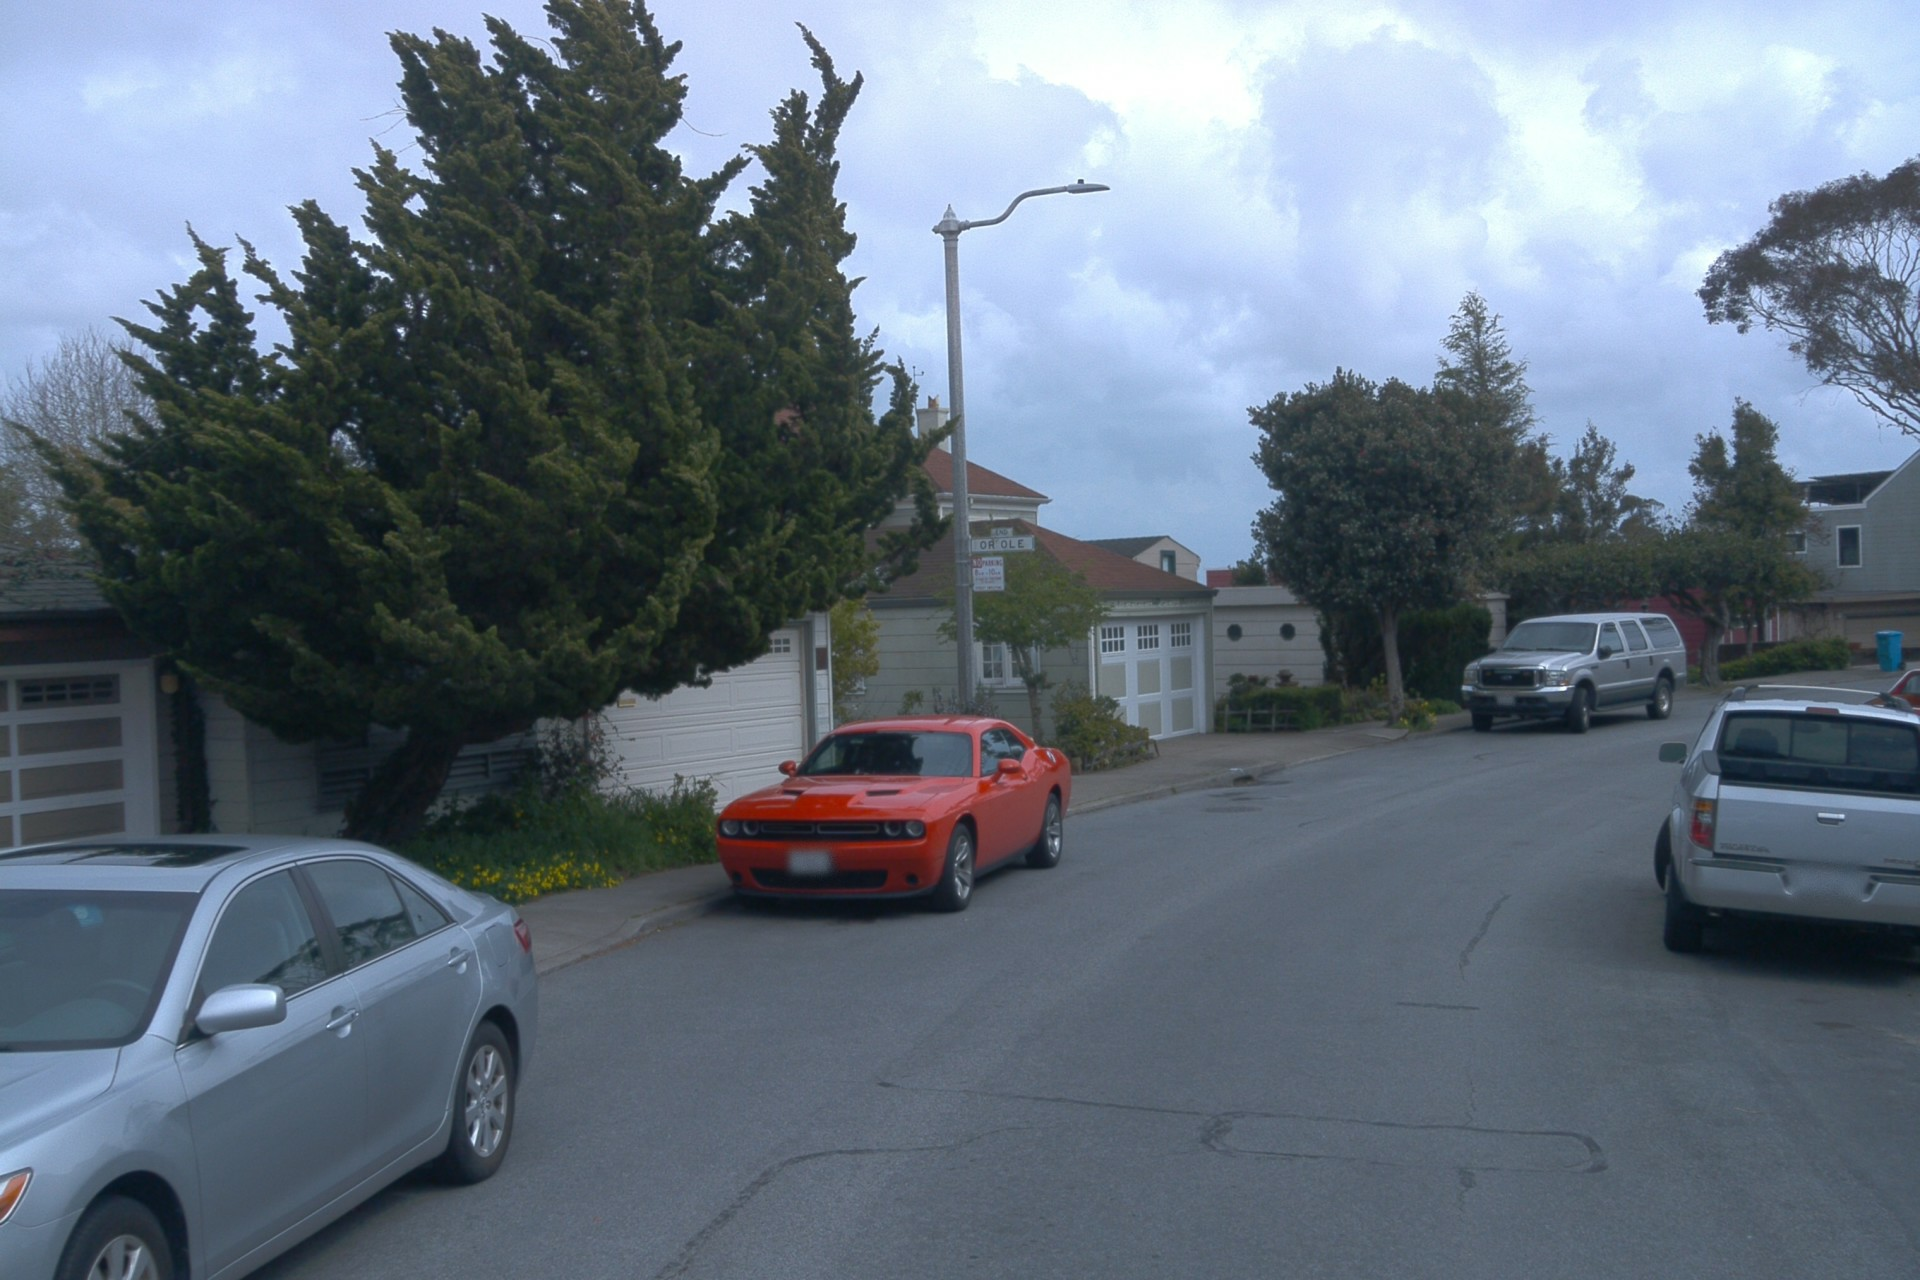
\includegraphics[width=.38\columnwidth, trim={0cm 0cm 0cm 0cm},clip]{fig/optimization_no_trunc_reg/scene2/gt_img.png}&
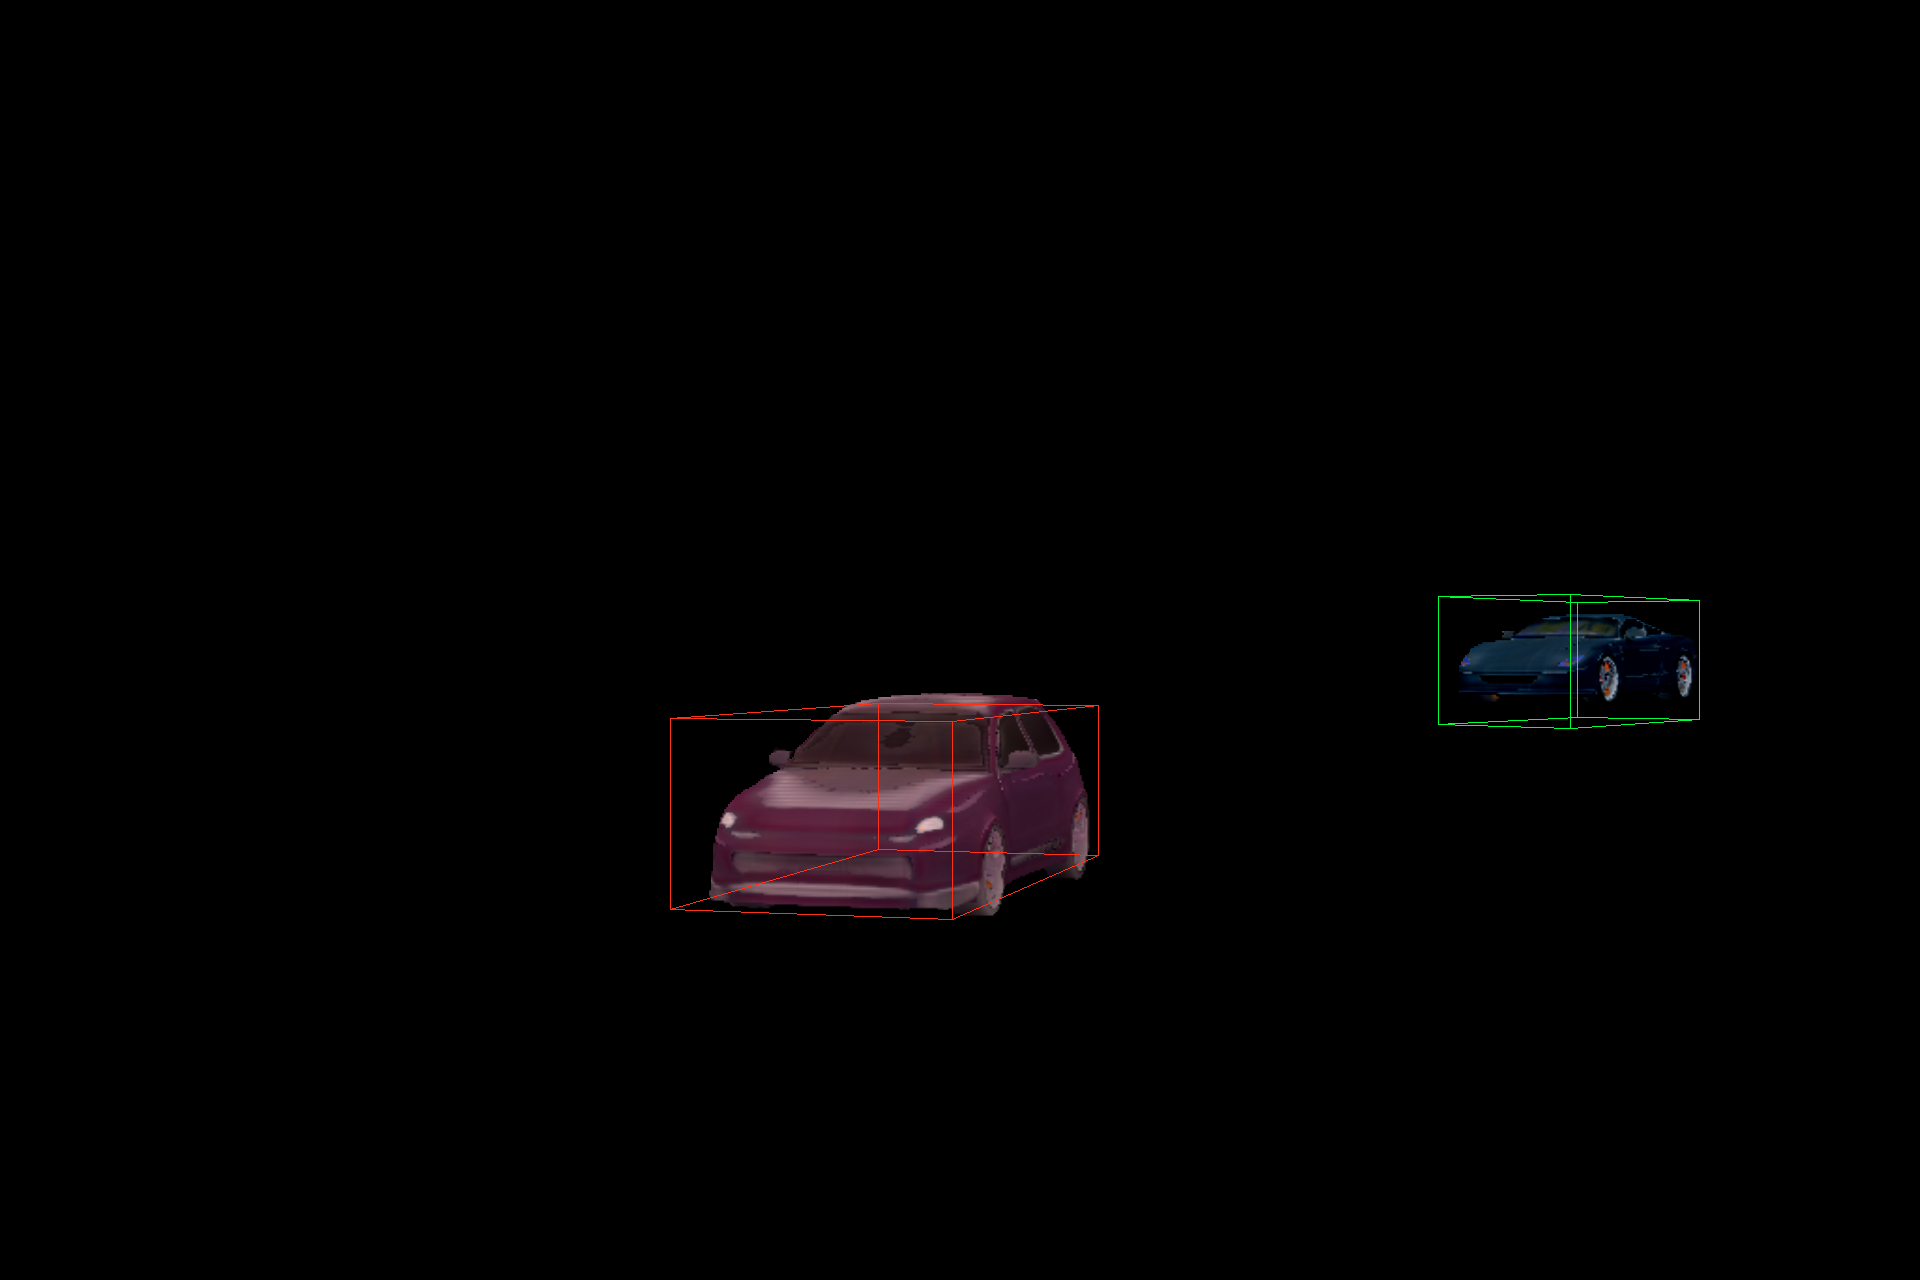
\includegraphics[width=.38\columnwidth, trim={0cm 0cm 0cm 0cm},clip]{fig/optimization_no_trunc_reg/scene2/noembed.png}&
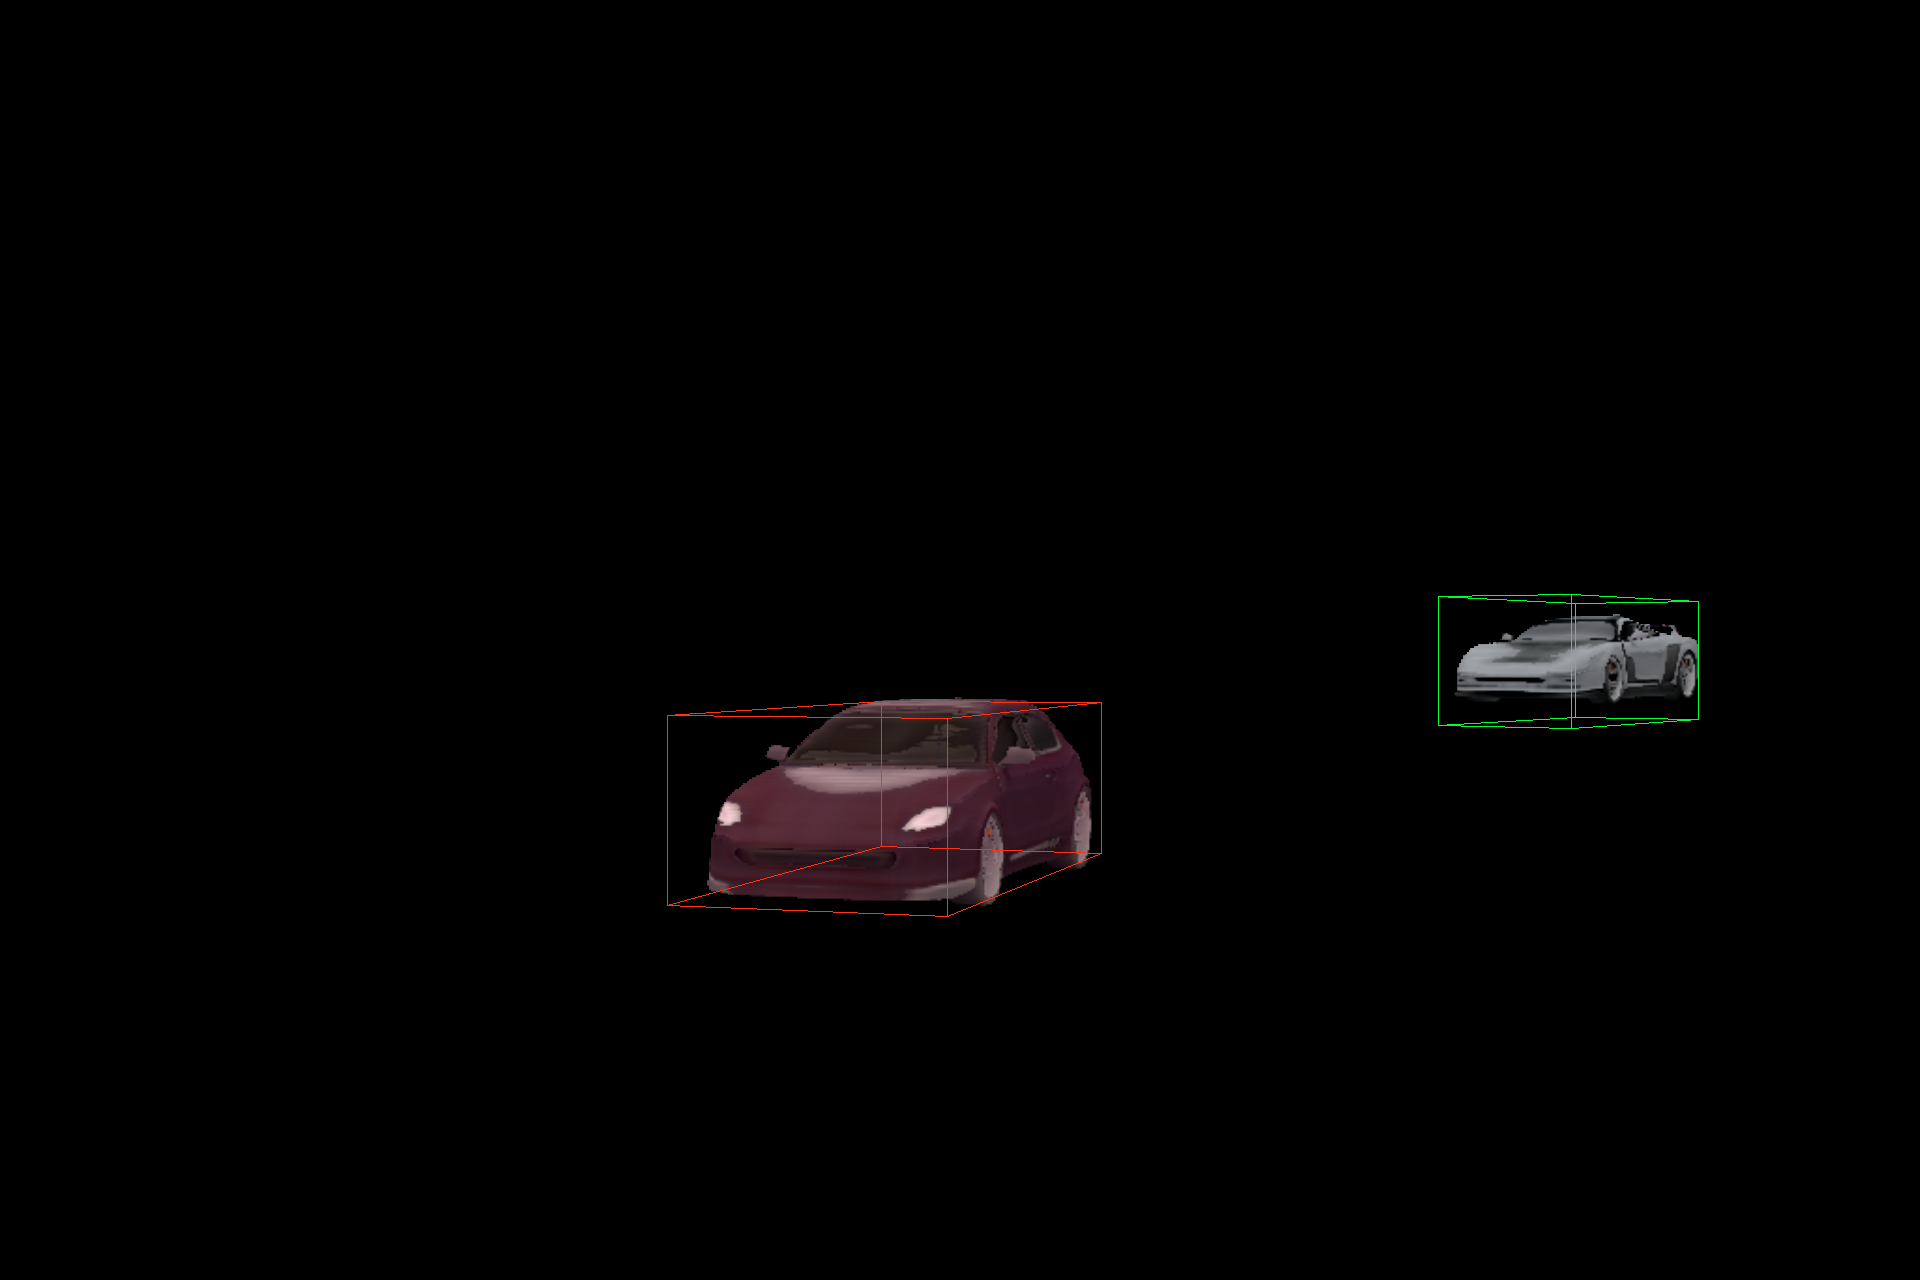
\includegraphics[width=.38\columnwidth, trim={0cm 0cm 0cm 0cm},clip]{fig/optimization_no_trunc_reg/scene2/im_w_bbox_rgb_out.png}
\end{tabular}}
\caption{\textbf{Truncation Trick.} From left to right, (i) The input observed image, (ii) results without truncation regularize applied and (iii) results with a truncation regularize applied. For images (ii) and (iii), we also show bounding boxes for each object color-coded by the respective predicted object IDs. As shown here, applying the truncation regularizer helps us achieve more accurate textures and better shapes and colors for the predicted car surface by forcing the optimized embedding to be ``well behaved'', i.e., close to the distribution of latent embeddings seen during the training by our representation model.}
\label{fig:optimization_truncation}
\end{figure}



\subsubsection{Learned Perceptual Loss.}
The goal of the perceptual loss is to guide the inverse rendering to match the abstracted feature-level appearance of individual objects. We use the pre-trained LPIPS~\cite{zhang2018perceptual} loss with VGG16~\cite{simonyan2015deep} backbone for this, which operates on rectangular images with a minimum side length of 16 pixels. To consider objects individually we crop and resize patches from $\hat I_c$ for each object $p$ respectively. Mask $M_{c,p} (i, j)$ describes all pixels rendered from each object with their respective index $i, j$. $M_{c,p} (i, j) = 1$ if object $p$ is projected into the respective pixel $i,j$ from camera $c$. We then can describe an image patch by its top and bottom corner. The patch top corner is defined as $\left( u_{top}, v_{top}\right) = \left( i_{min, M_{c,p}}, j_{min, M_{c,p}}\right)$, the upper and left corner of a tight axis-aligned rectangle around all rendered pixels. The patch bottom corner is defined as $\left( u_{bot}, v_{bot}\right) = \left( i_{max, M_{c,p}}, j_{max, M_{c,p}}\right)$, the lower and right corner of the same axis-aligned rectangle. \\
\subsubsection{Latent Embedding Regularization.}
%
Modern generative-adversarial (GAN)~\cite{karras2019styleGAN,karras2020styleGAN2,gao2022get3d,sauer2022styleganXL,kang2023gigaGAN} methods, such as the used 3D object generator~\cite{gao2022get3d} first map an embedding sample from a multivariate Gaussian, called z-space or distribution, into a learned embedding space, called w-space, following a different distribution. The intuition behind this is that there are more optimal embedding distributions, which can be more easily mapped to the data distribution that the GAN is generating. High-quality samples are only generated from embeddings inside the high-dimensional embedding distribution. Therefore, we regularize the optimized embedding code through inverse rendering, with
\begin{equation}
    \mathcal{L}_{embed} = \alpha_T\mathbf{z}_T + (1 - \alpha_T)\mathbf{z}_T^{avg} +  \alpha_S\mathbf{z}_S + (1 - \alpha_S)\mathbf{z}_S^{avg},
\end{equation}
that is Eq.(14) in the main paper. Here, $\alpha_T$ and $\alpha_S$ are set to $0.7$.

We employ the \emph{truncation trick} widely used in GAN-based generators and first presented in StyleGAN~\cite{karras2019styleGAN}, where $z^{avg}$ represents an exponential-moving average of embedding codes generated from the Gaussian training during the training of the generator. This stabilizes the optimization through inverse rendering as Fig.~\ref{fig:optimization_truncation} shows.



\subsubsection{Weighting}
With empirical analysis of the validation set of both datasets, we find the weighting of loss terms $\lambda_1 = 0.4$, $\lambda_2 = 3$, and $\lambda_3 = 10$ for stable and truthfully generated objects via inverse rendering.




\subsection{Optimization Schedule}
For the loss function presented in Eq.~(5) of the main paper, we found that the schedule presented in Tab.~\ref{tab:schedule} solves this optimization problem effectively, while being stable across various scenes and datasets.

We first fit the texture embedding in only three steps during the test-time optimization of all object parameters. In step 3, we jointly solve for pose, scale, and shape, followed by three more steps on shape only. Details on the learning rate for the respective parameters are reported in Tab.~\ref{tab:schedule}.

An exhaustive search is impossible due to the number of hyper-parameters when including different loss functions and terms. We therefore performed empirical investigation on small, diverse subsets of scenes to find the parameter set used. The same setting works well on all datasets and \emph{have not been changed} for the Waymo Open Dataset~\cite{sun2020scalability} and the nuScenes dataset~\cite{caesar2020nuscenes}.

% \begin{figure*}[t!]
	% \vspace{-12pt}
	% \renewcommand{\arraystretch}{0.5}
\centering
\resizebox{0.98\linewidth}{!}{%
\begin{tabular}{@{}c@{\hskip .1cm}c@{\hskip .1cm}c@{\hskip .1cm}c@{\hskip .1cm}c@{}}
{\small Input Frame} & {\small Initial Guess} & {\small Texture Fitting} & {\small Object Pose Fitting} &{\small Shape Fitting} \\
	    
% 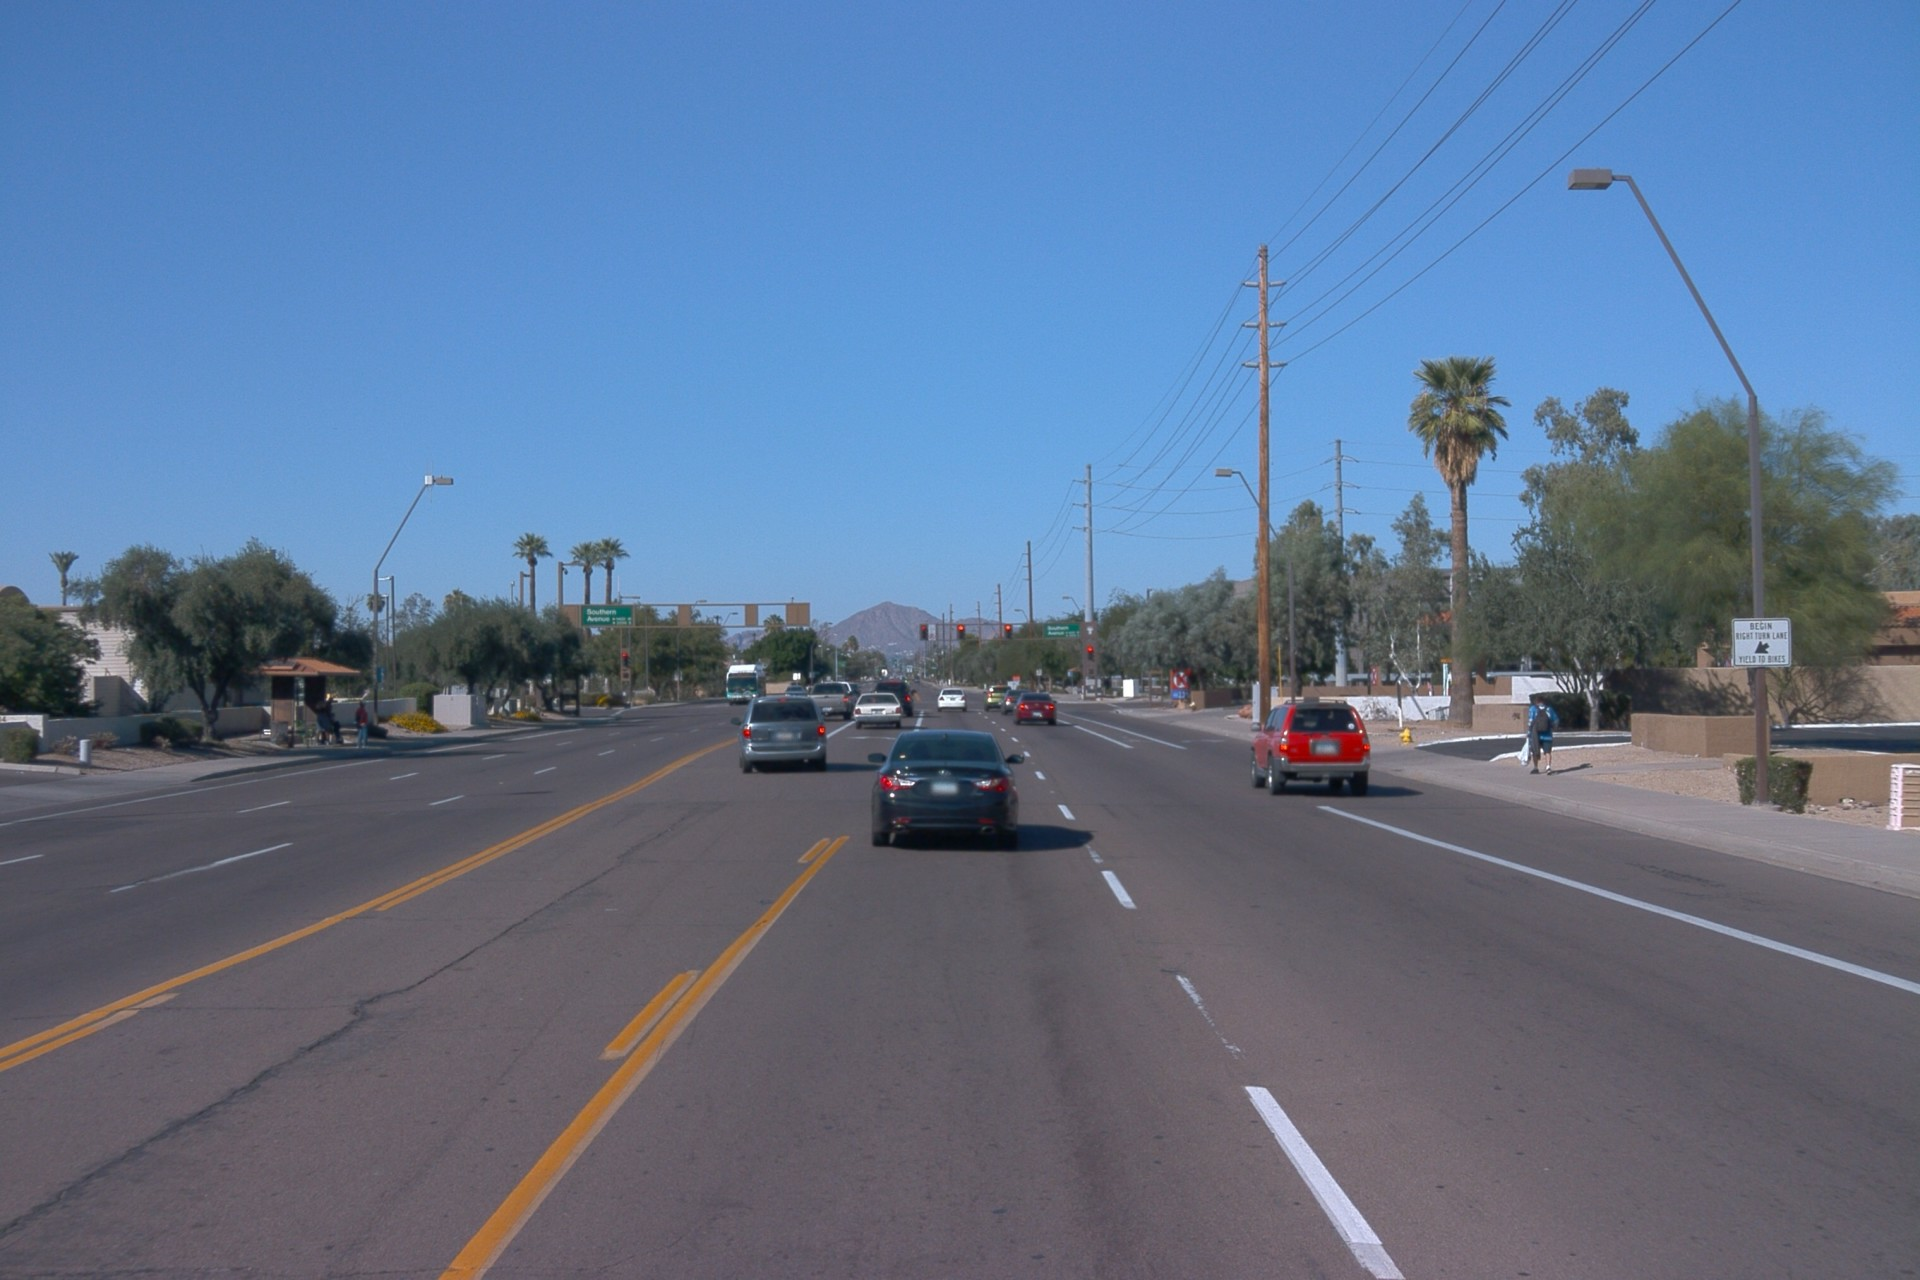
\includegraphics[width=.44\columnwidth, trim={0cm 0cm 0cm 0cm},clip]{fig/optim_supplement/scene50/initial_guess_50_10_waymo.png}&
% 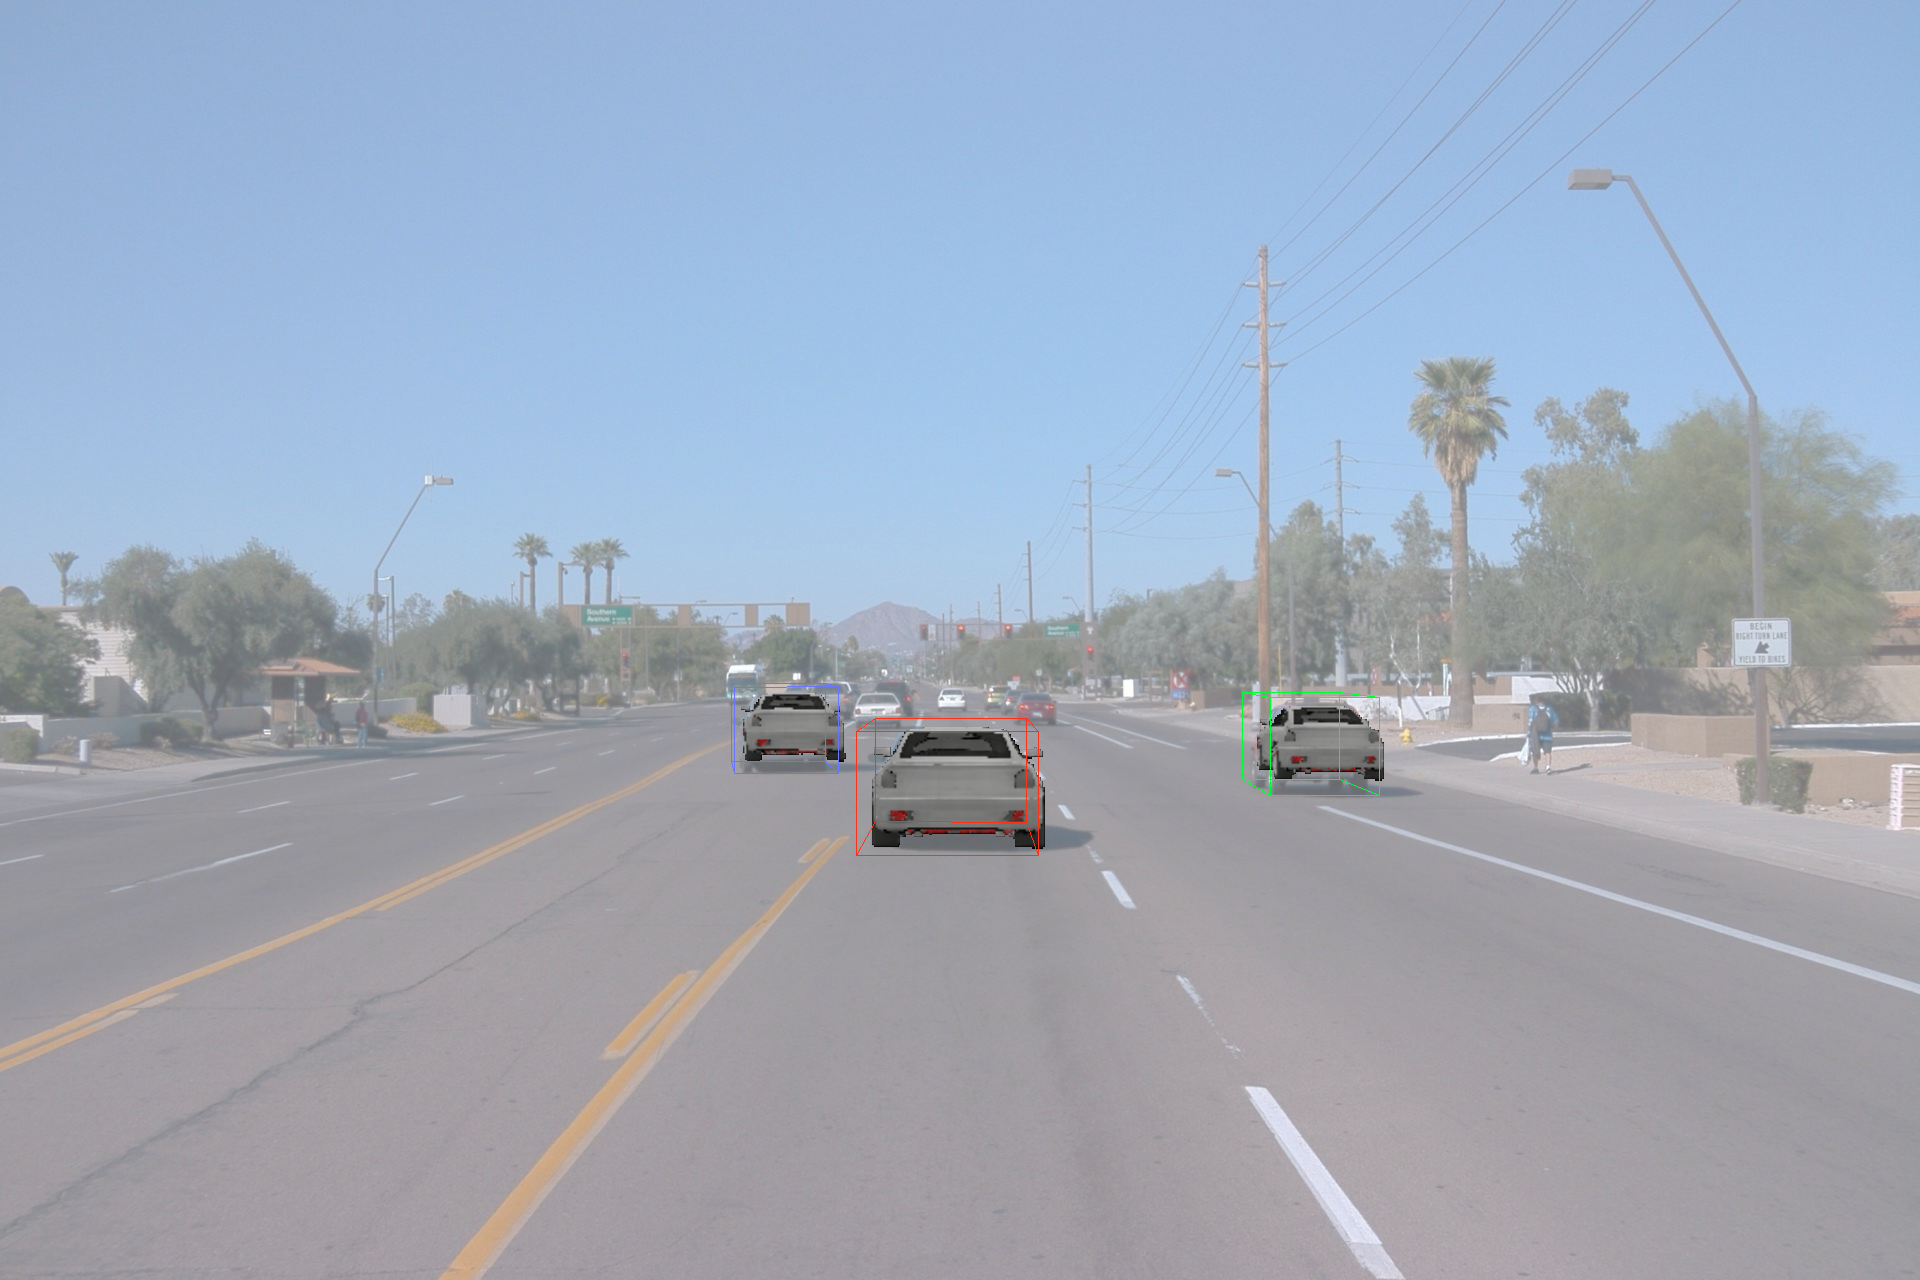
\includegraphics[width=.44\columnwidth, trim={0cm 0cm 0cm 0cm},clip]{fig/optim_supplement/scene50/init_guess-50.png}&
% 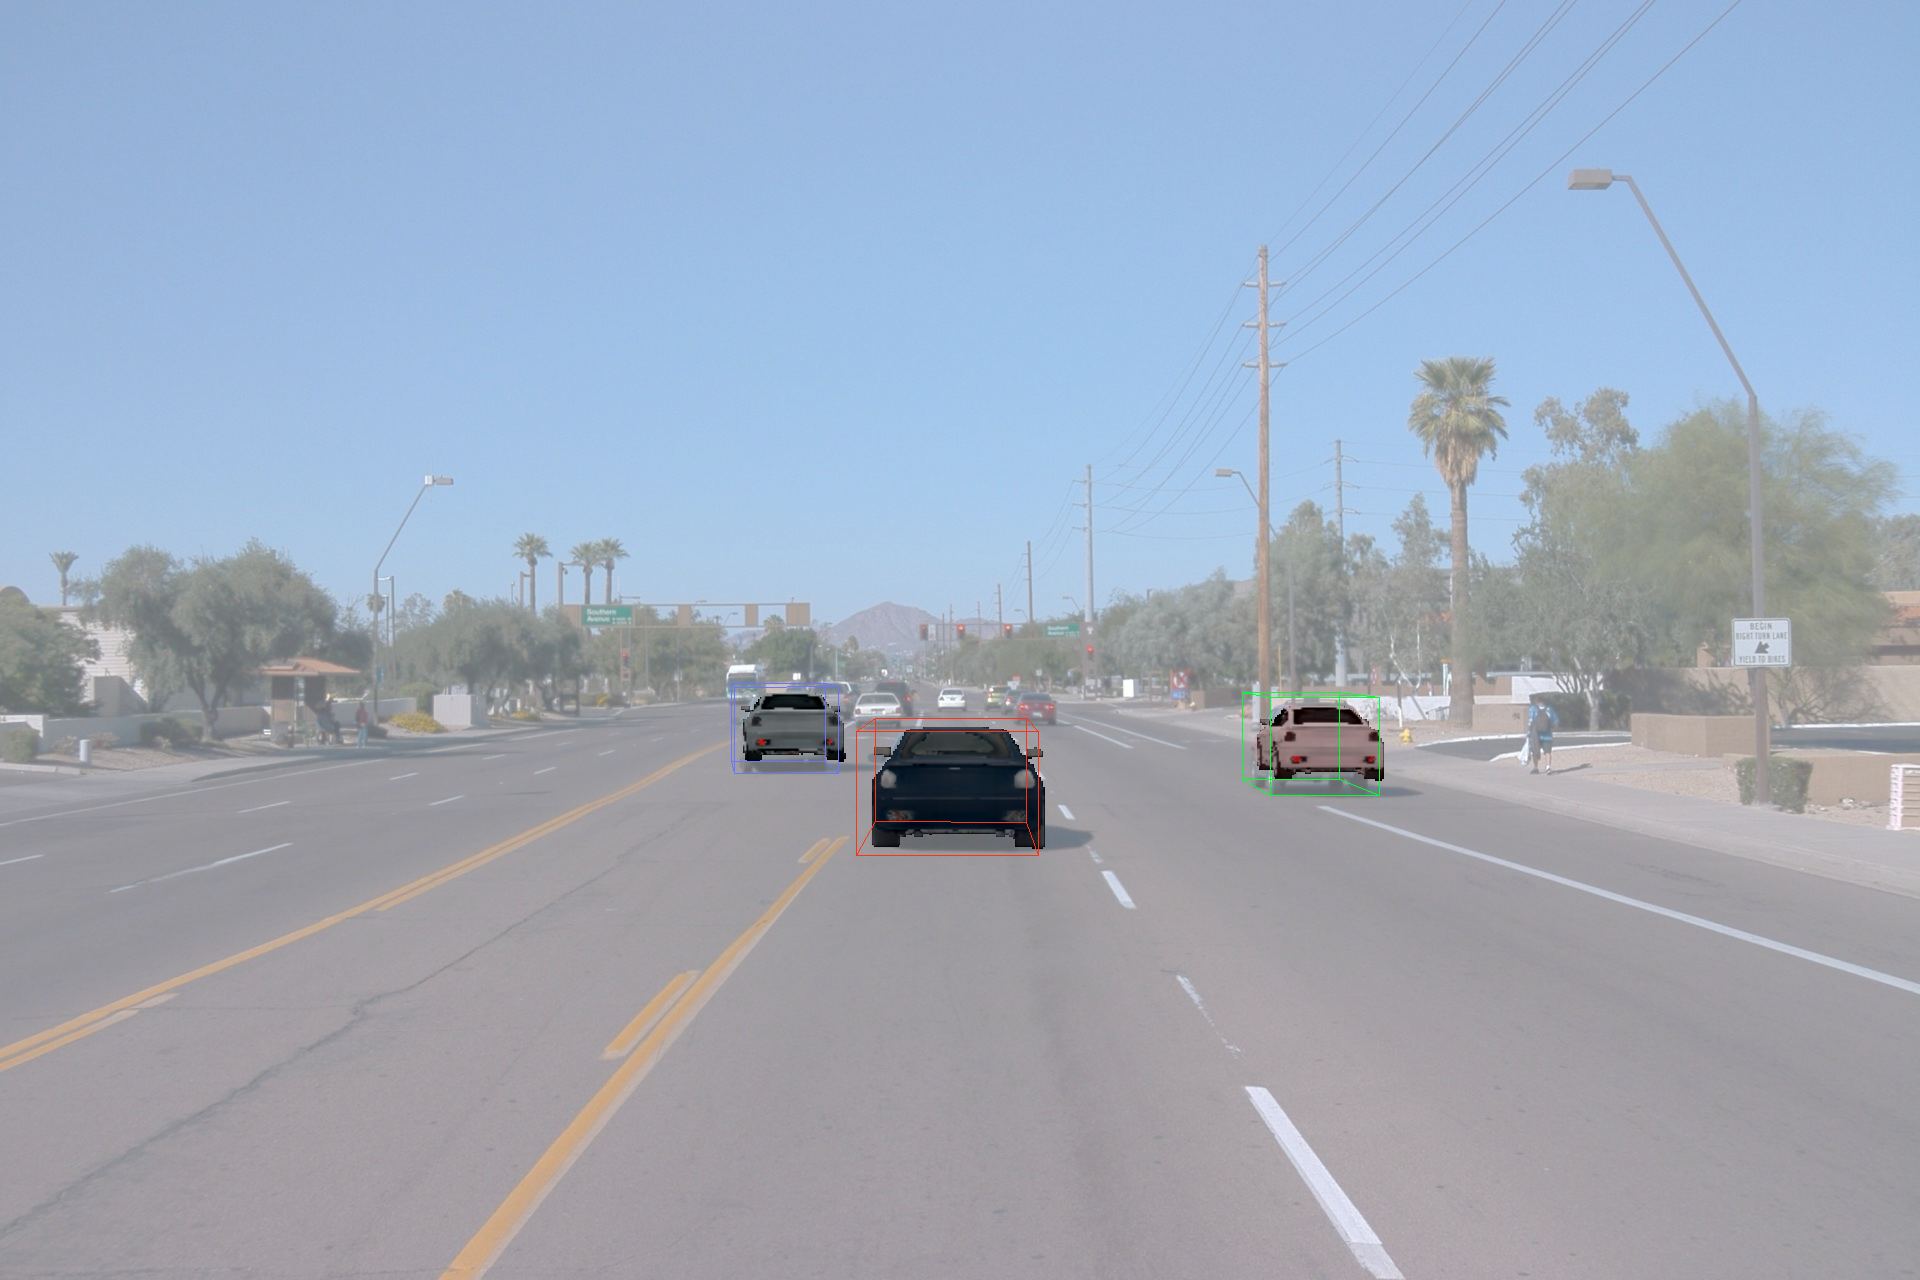
\includegraphics[width=.44\columnwidth, trim={0cm 0cm 0cm 0cm},clip]{fig/optim_supplement/scene50/tex_50_10.png}&
% 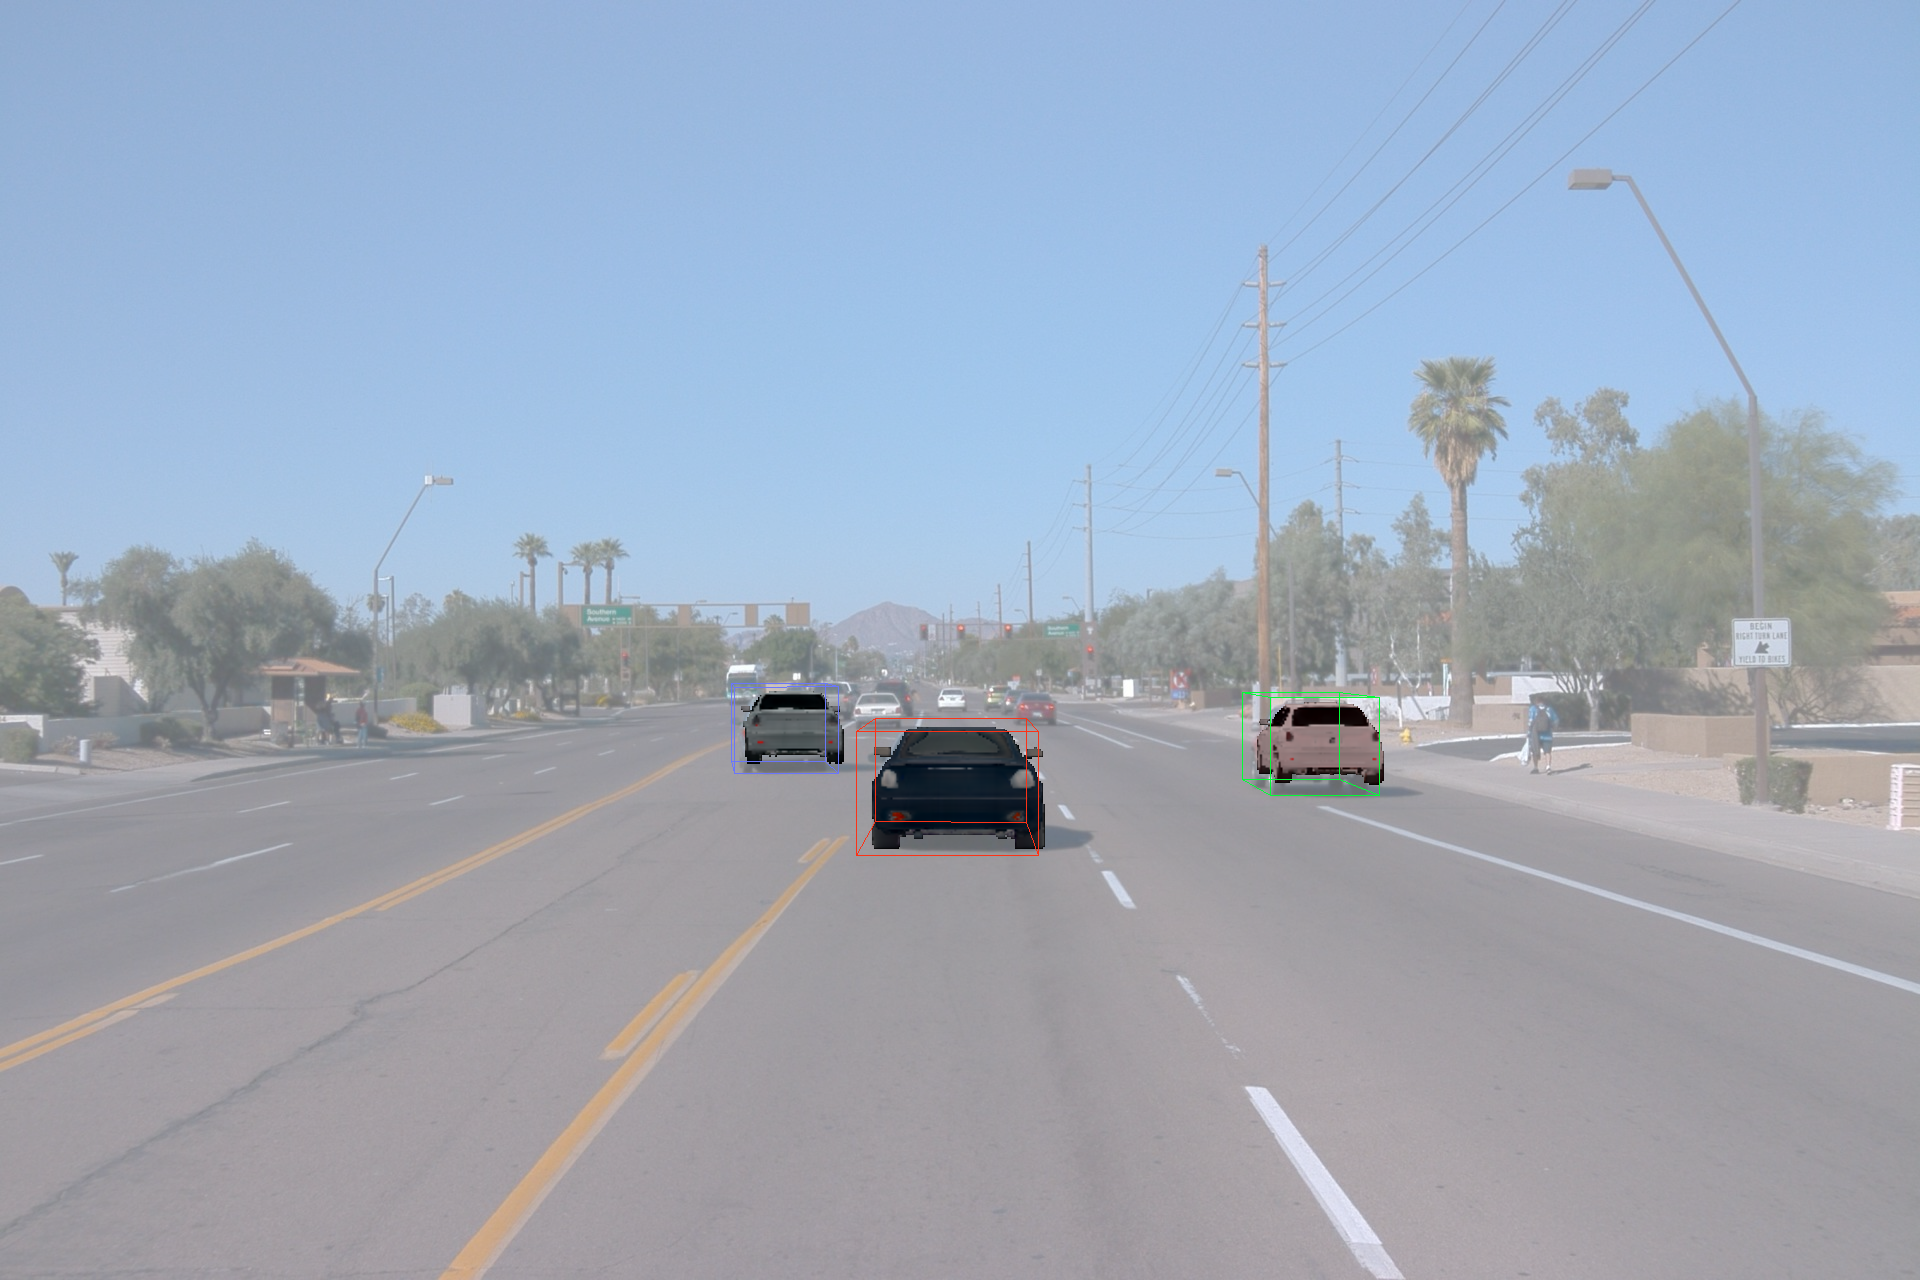
\includegraphics[width=.44\columnwidth, trim={0cm 0cm 0cm 0cm},clip]{fig/optim_supplement/scene50/4_50_10.png}&
% 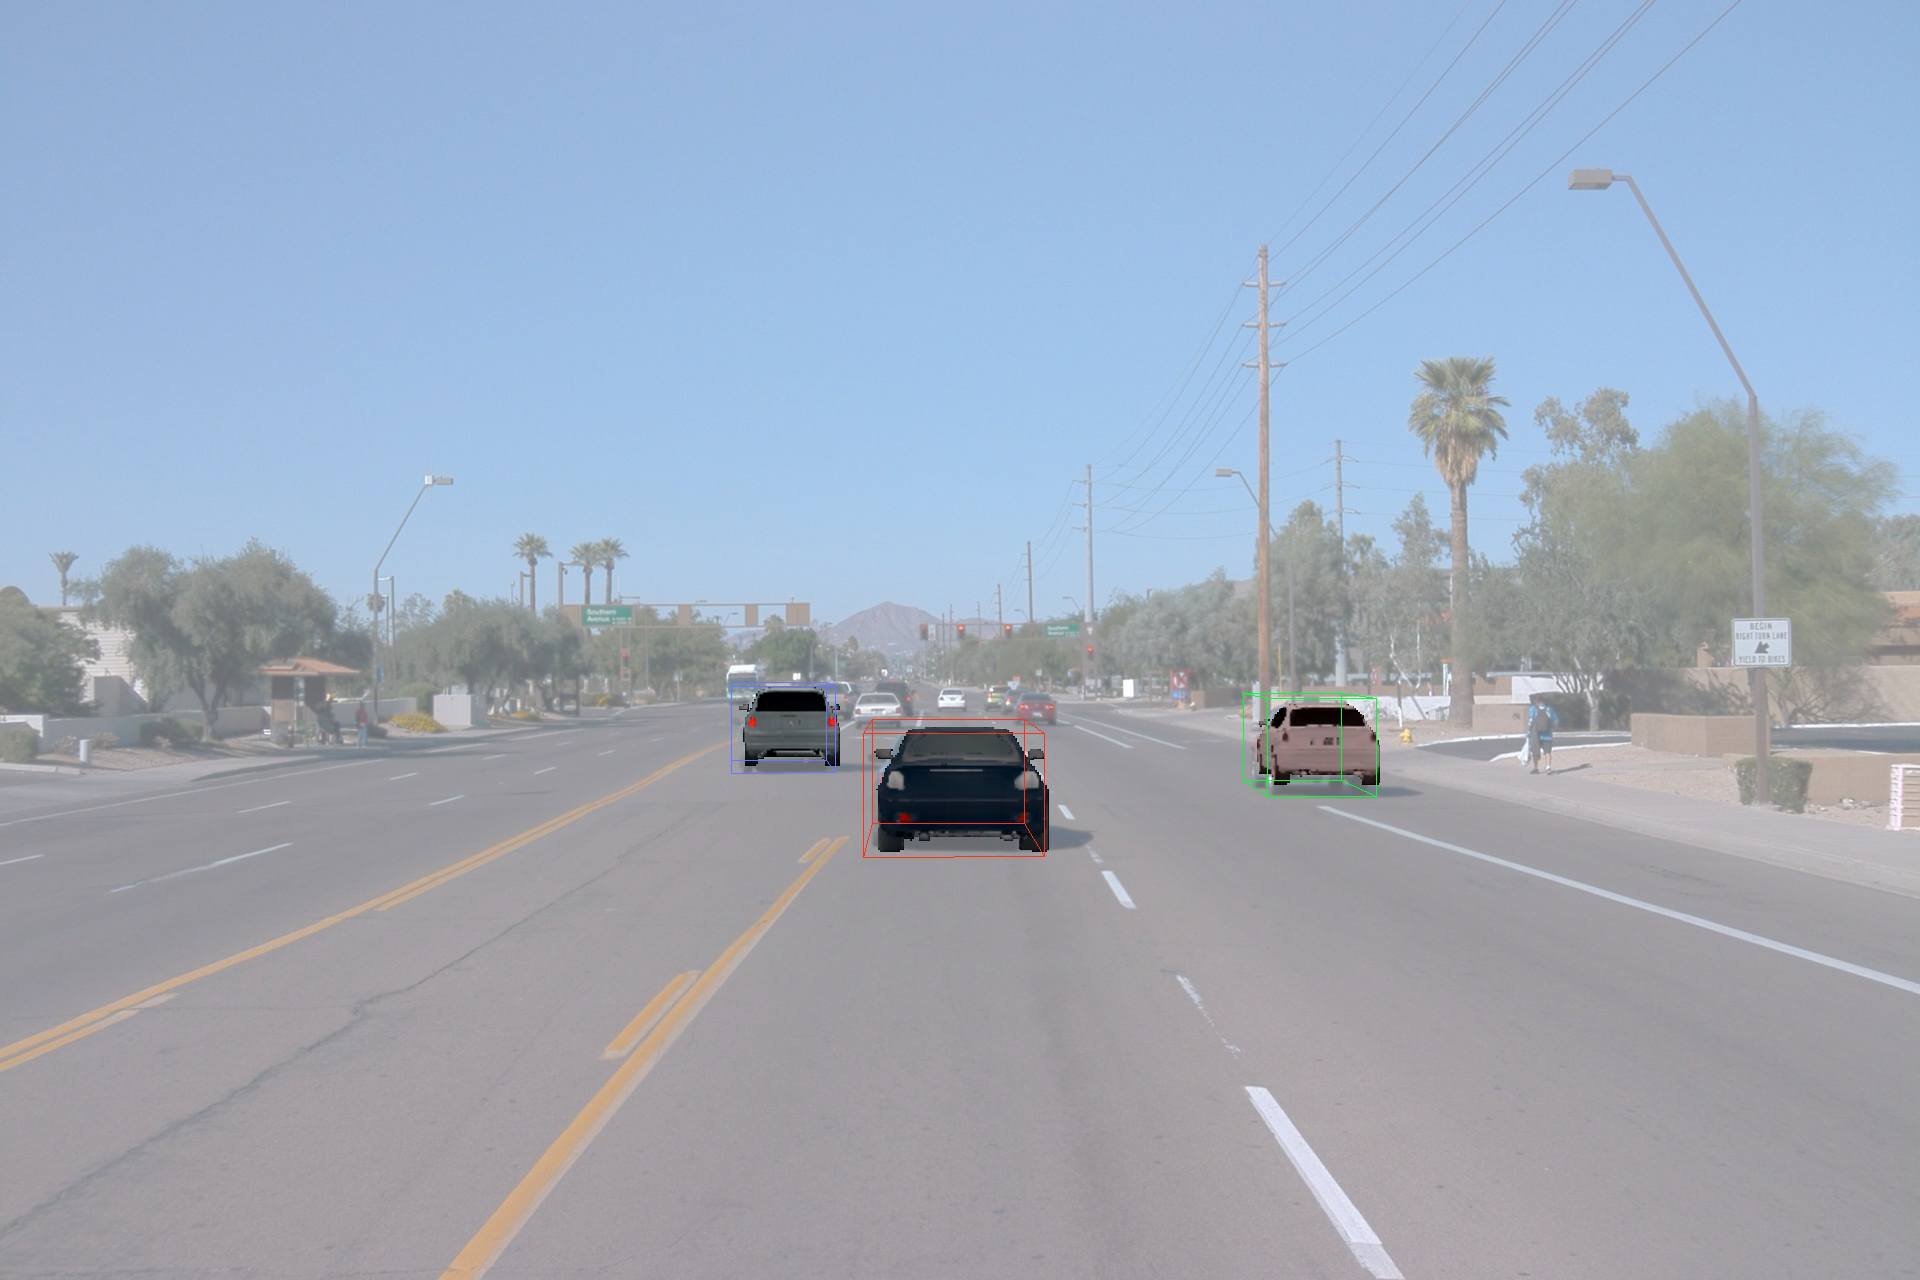
\includegraphics[width=.44\columnwidth, trim={0cm 0cm 0cm 0cm},clip]{fig/optim_supplement/scene50/5_50_10.png} \\

% 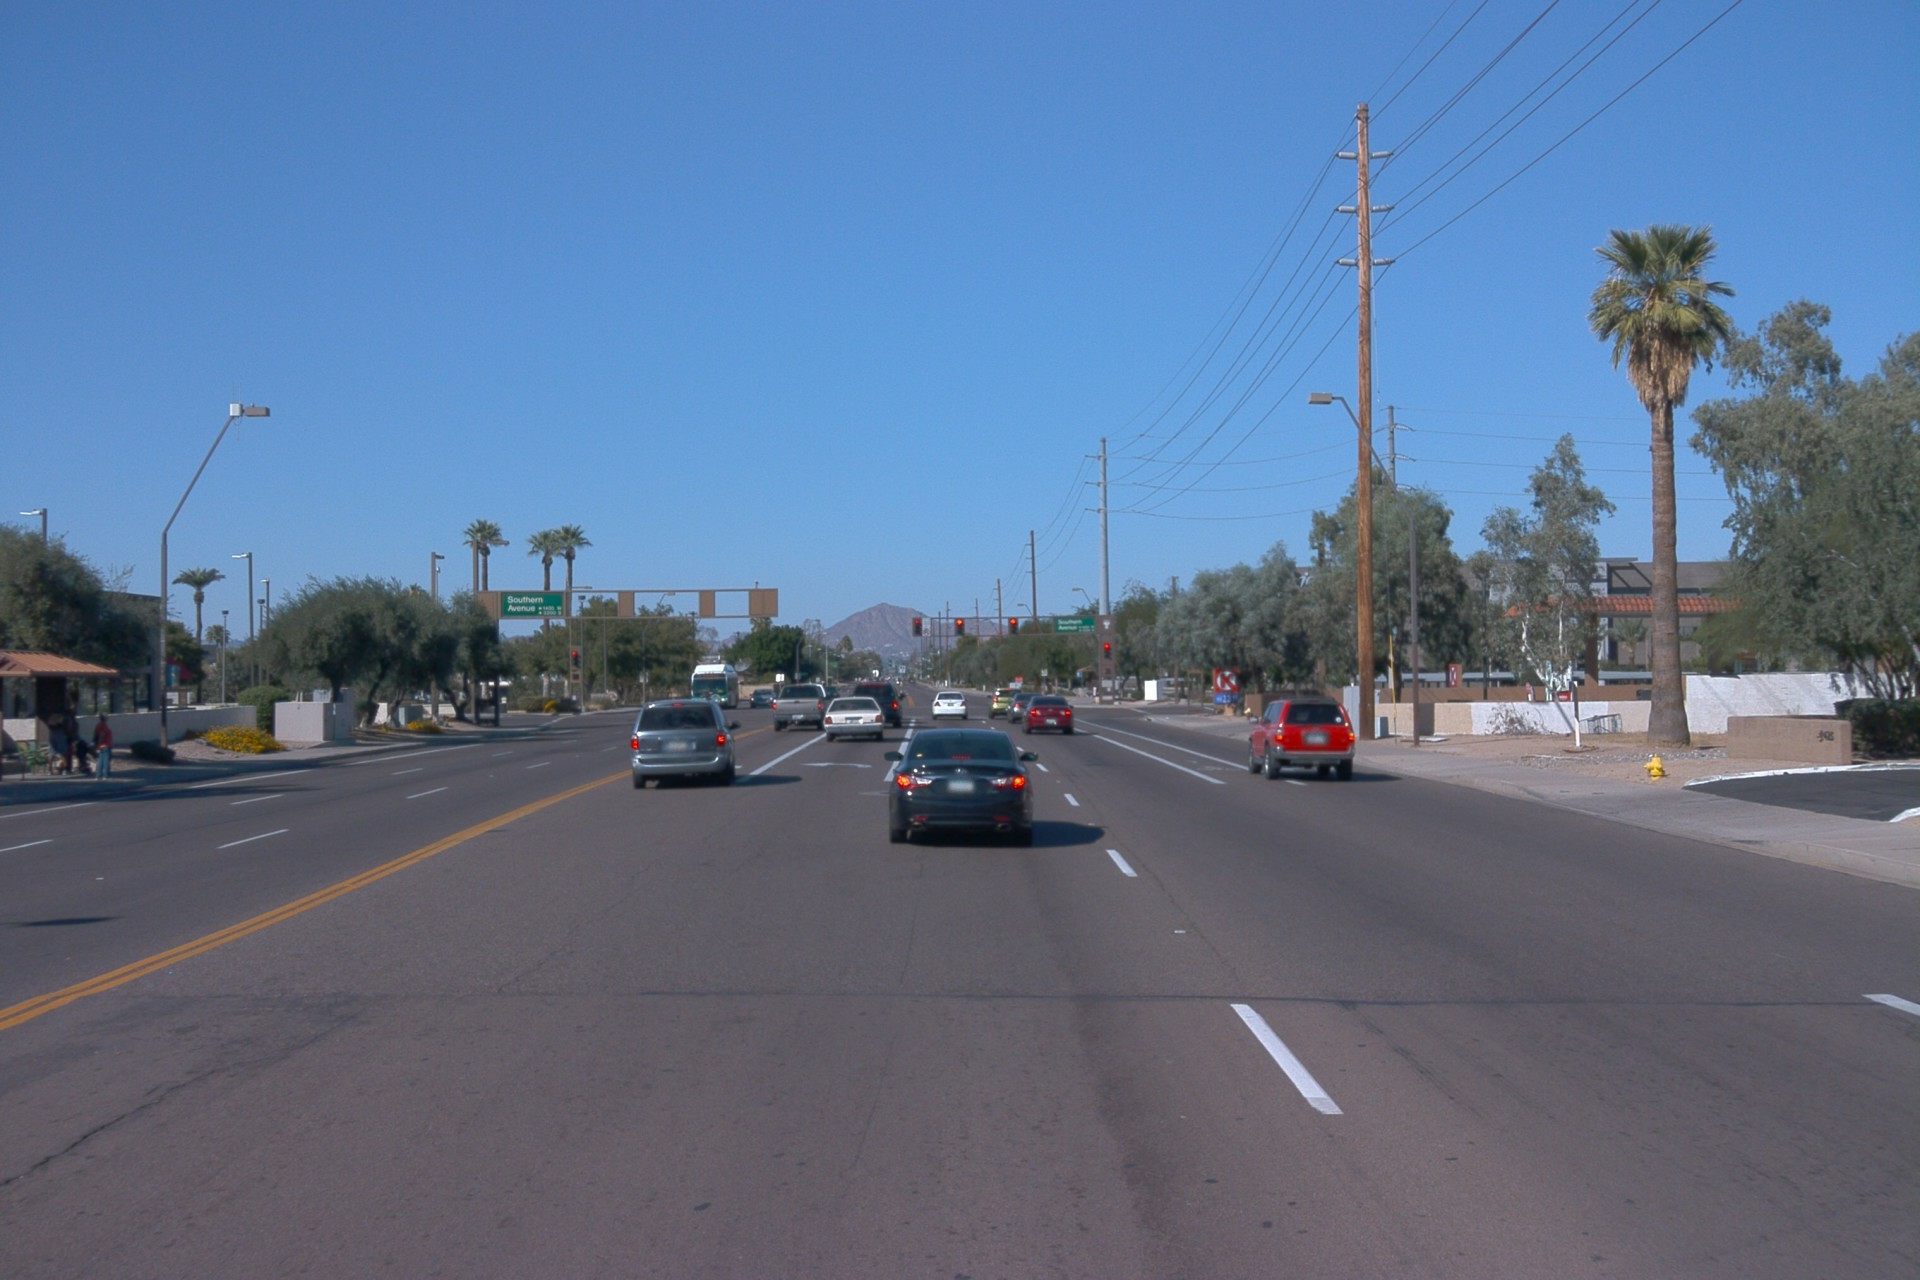
\includegraphics[width=.44\columnwidth, trim={0cm 0cm 0cm 0cm},clip]{fig/optim_supplement/scene50_26/50_26_gt.png}&
% 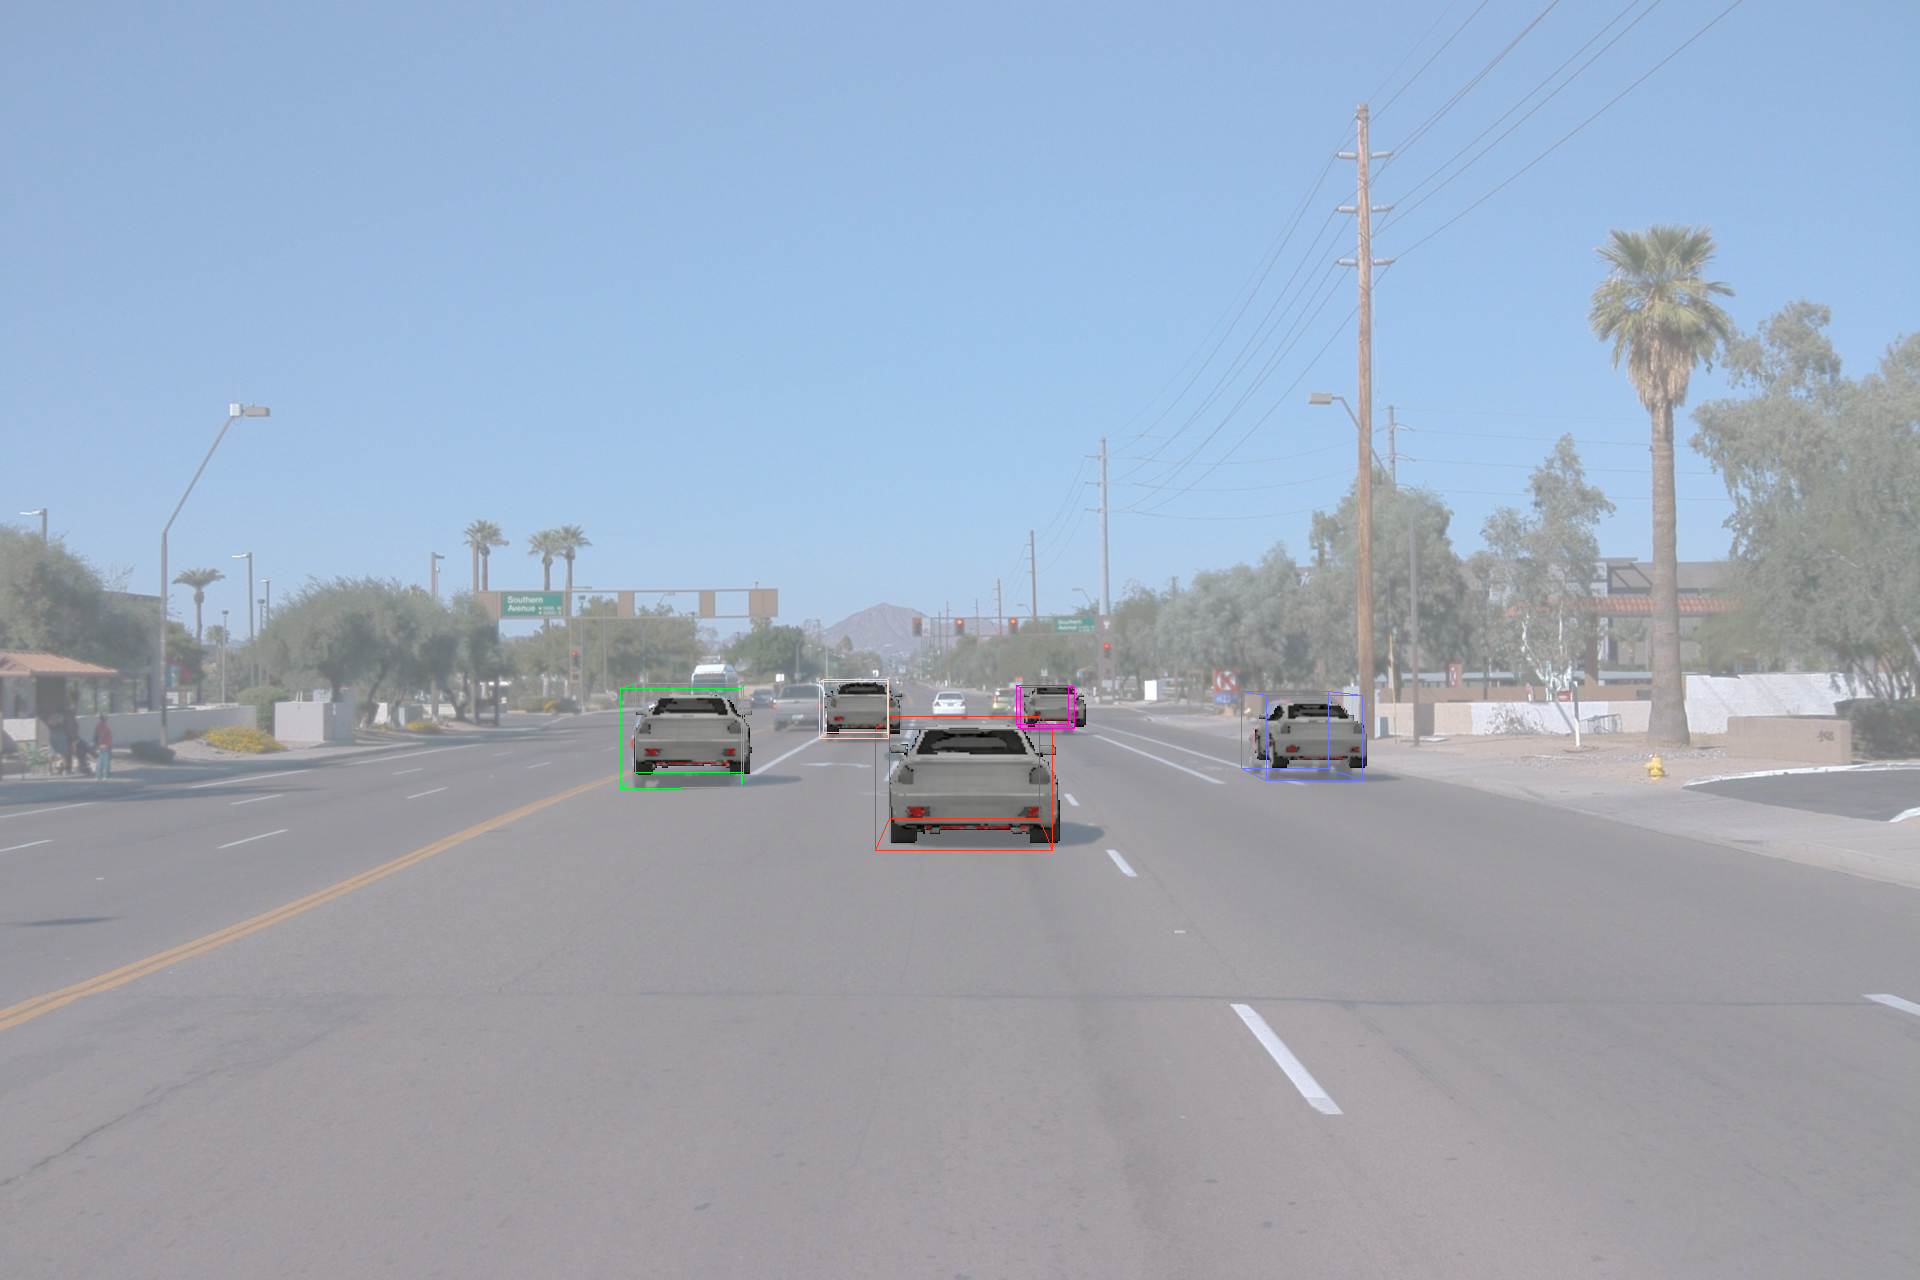
\includegraphics[width=.44\columnwidth, trim={0cm 0cm 0cm 0cm},clip]{fig/optim_supplement/scene50_26/50_26_0.png}&
% 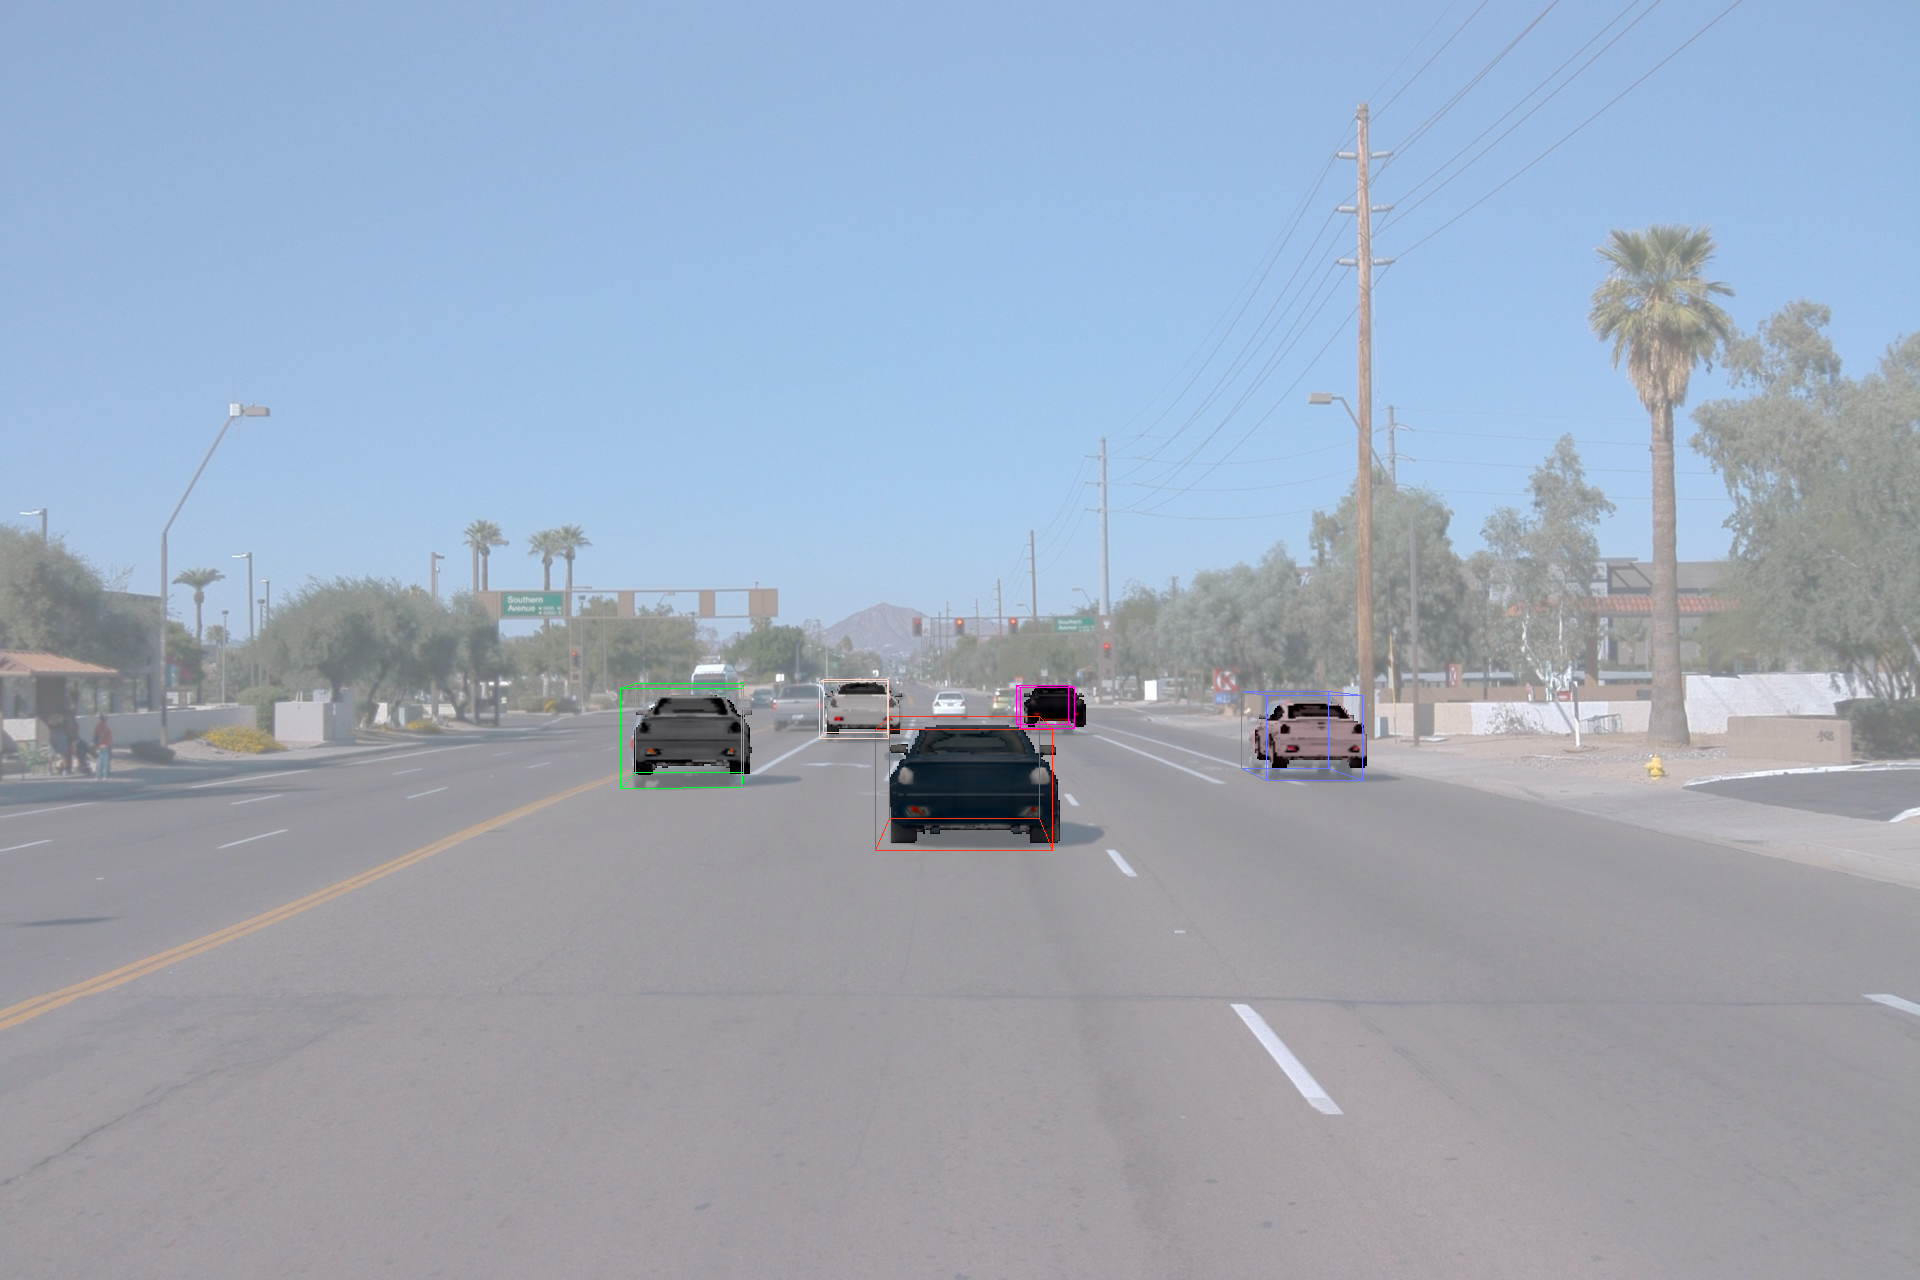
\includegraphics[width=.44\columnwidth, trim={0cm 0cm 0cm 0cm},clip]{fig/optim_supplement/scene50_26/50_26_3.png}&
% 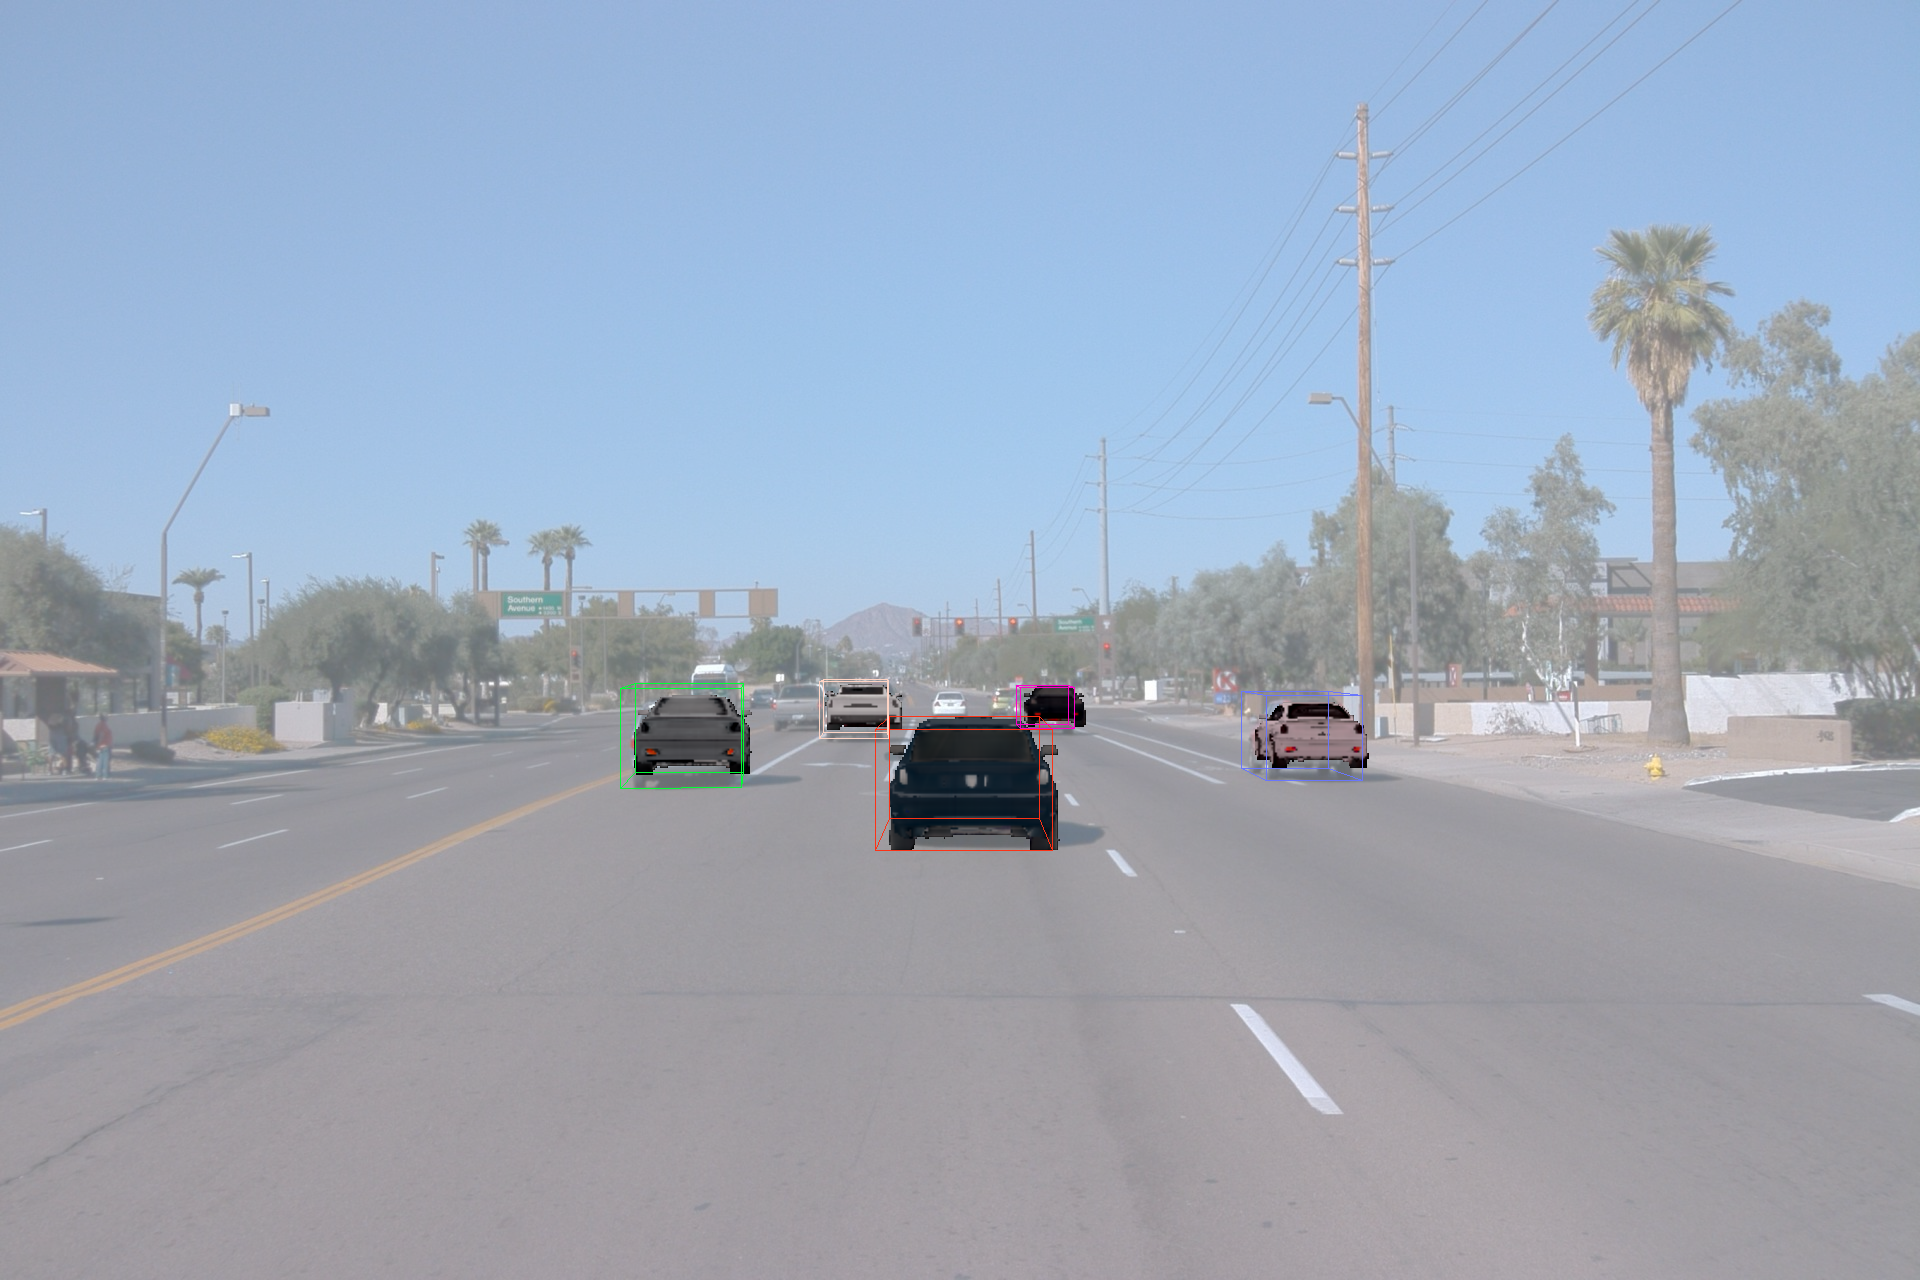
\includegraphics[width=.44\columnwidth, trim={0cm 0cm 0cm 0cm},clip]{fig/optim_supplement/scene50_26/50_26_4.png}&
% 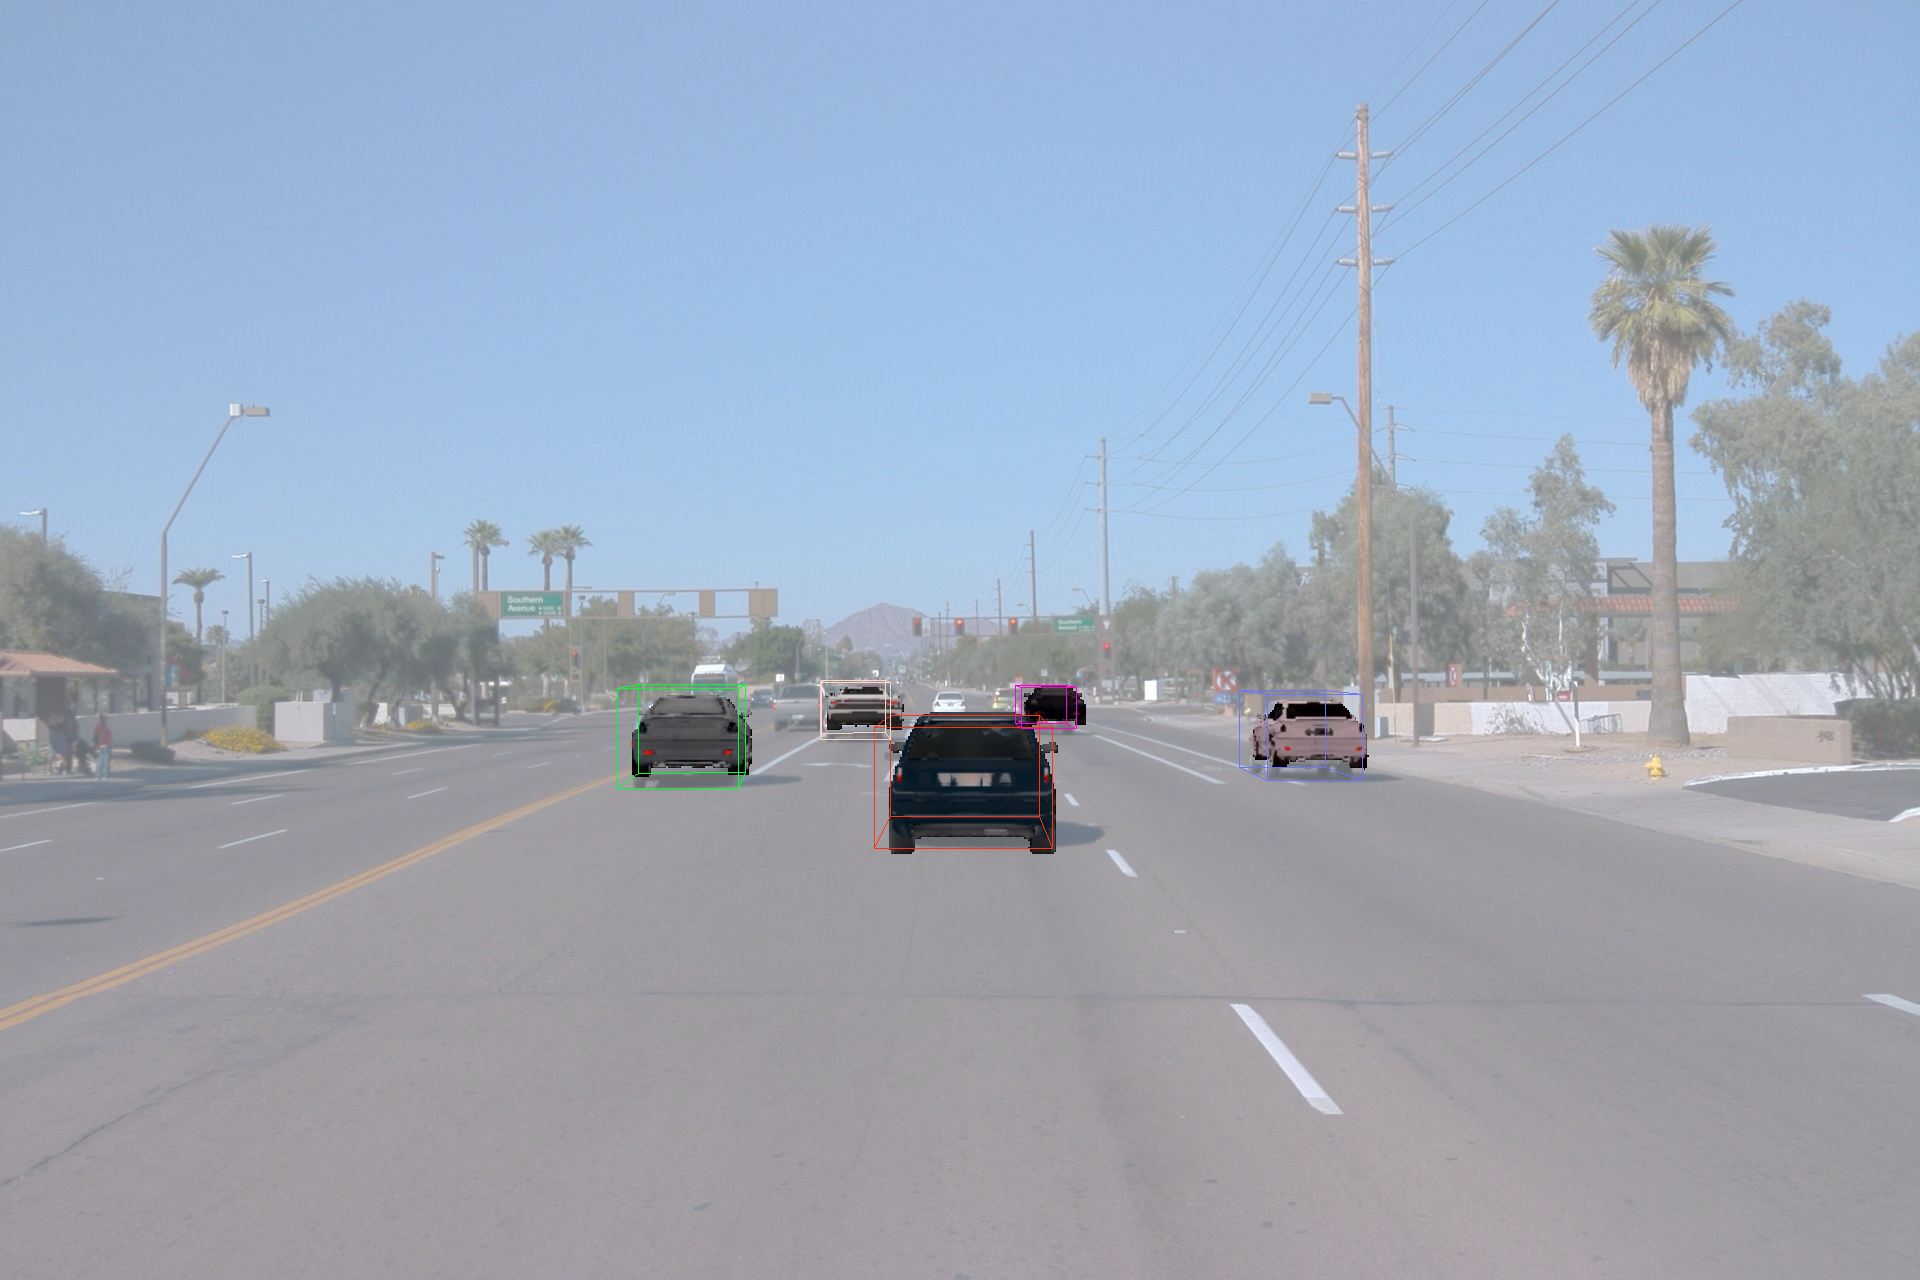
\includegraphics[width=.44\columnwidth, trim={0cm 0cm 0cm 0cm},clip]{fig/optim_supplement/scene50_26/50_26_5.png} \\

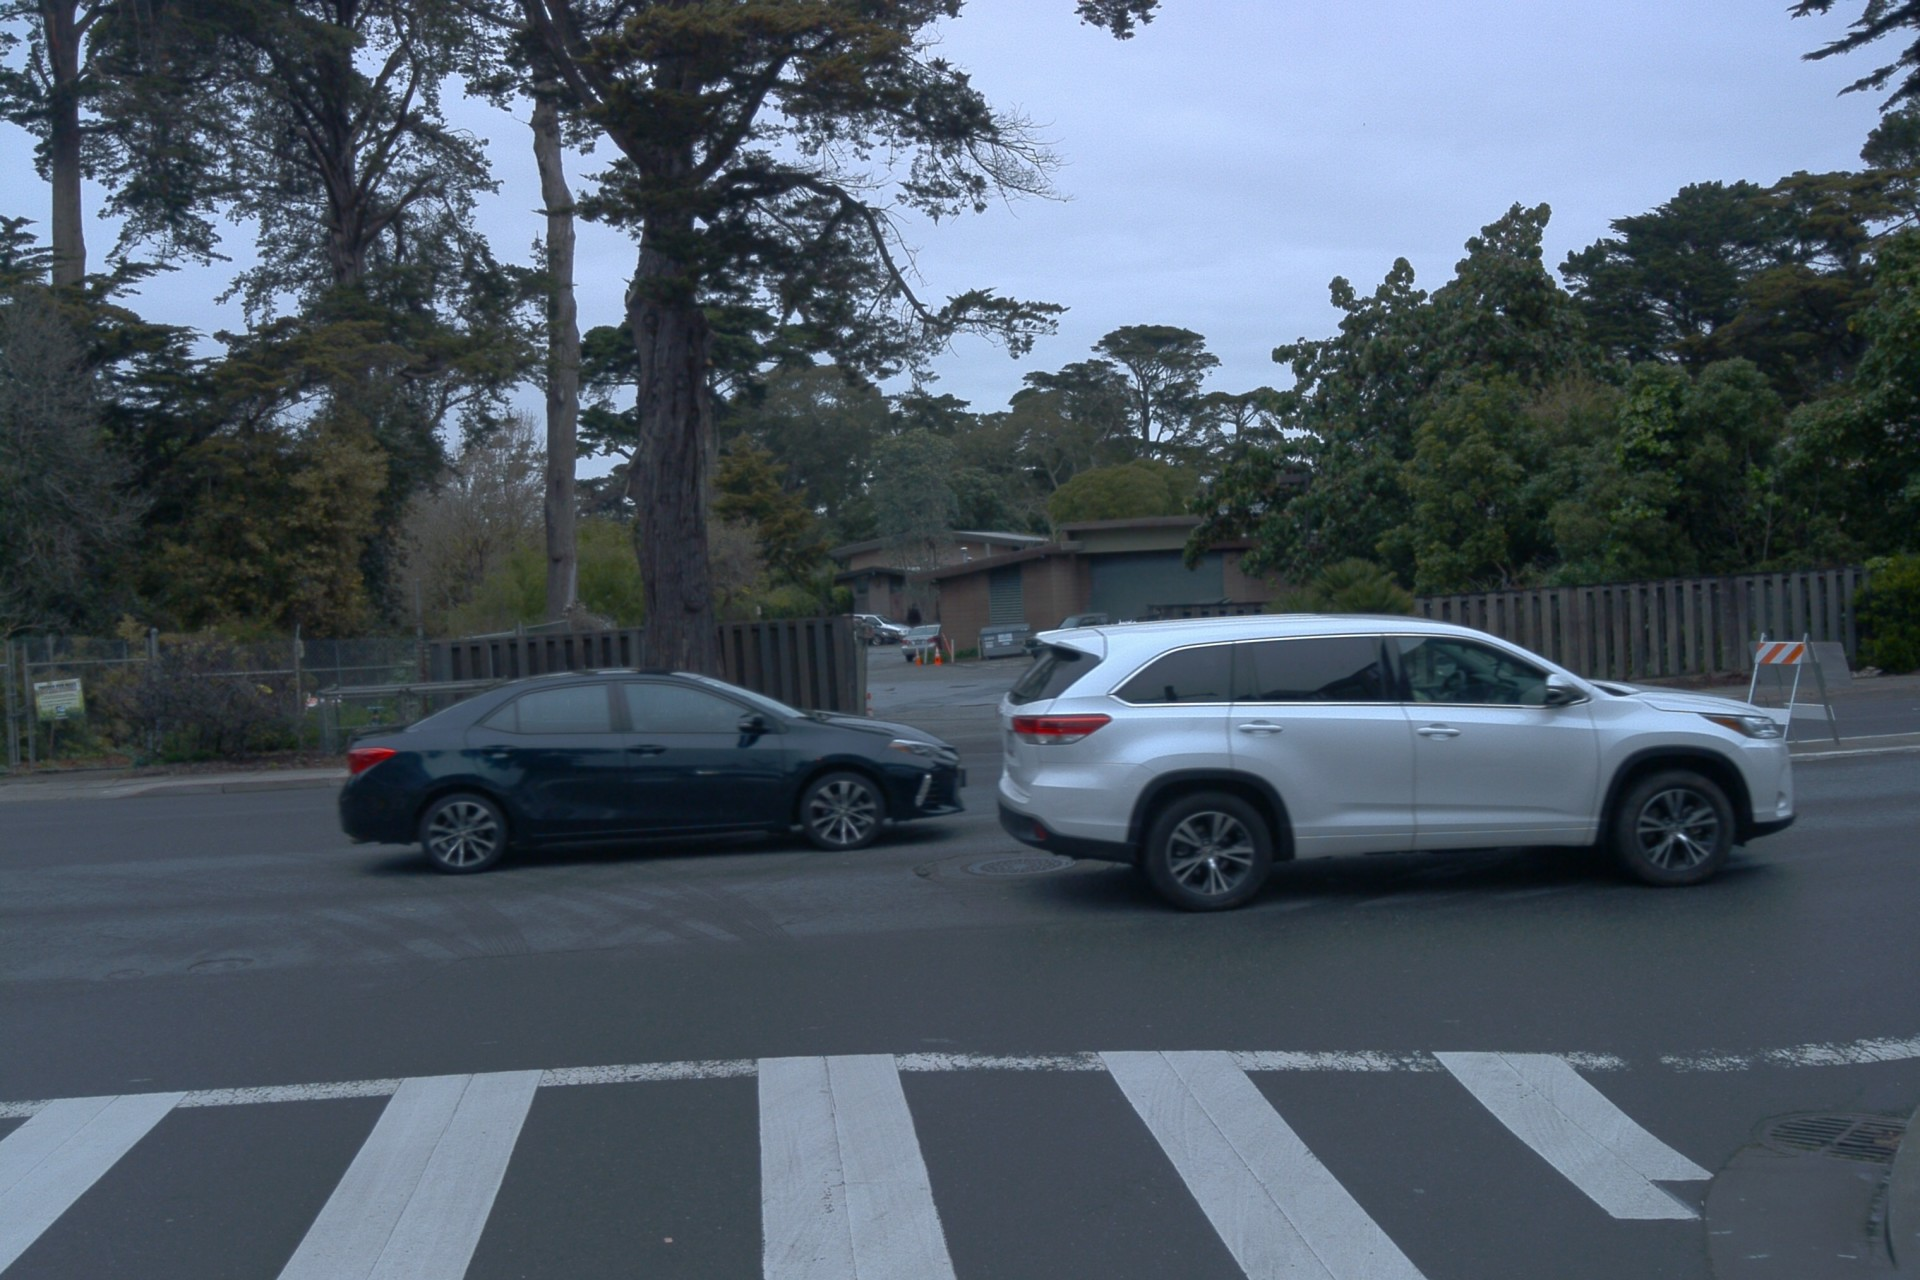
\includegraphics[width=.44\columnwidth, trim={0cm 0cm 0cm 0cm},clip]{fig/optim_supplement/scene11_104/gt_img.png}&
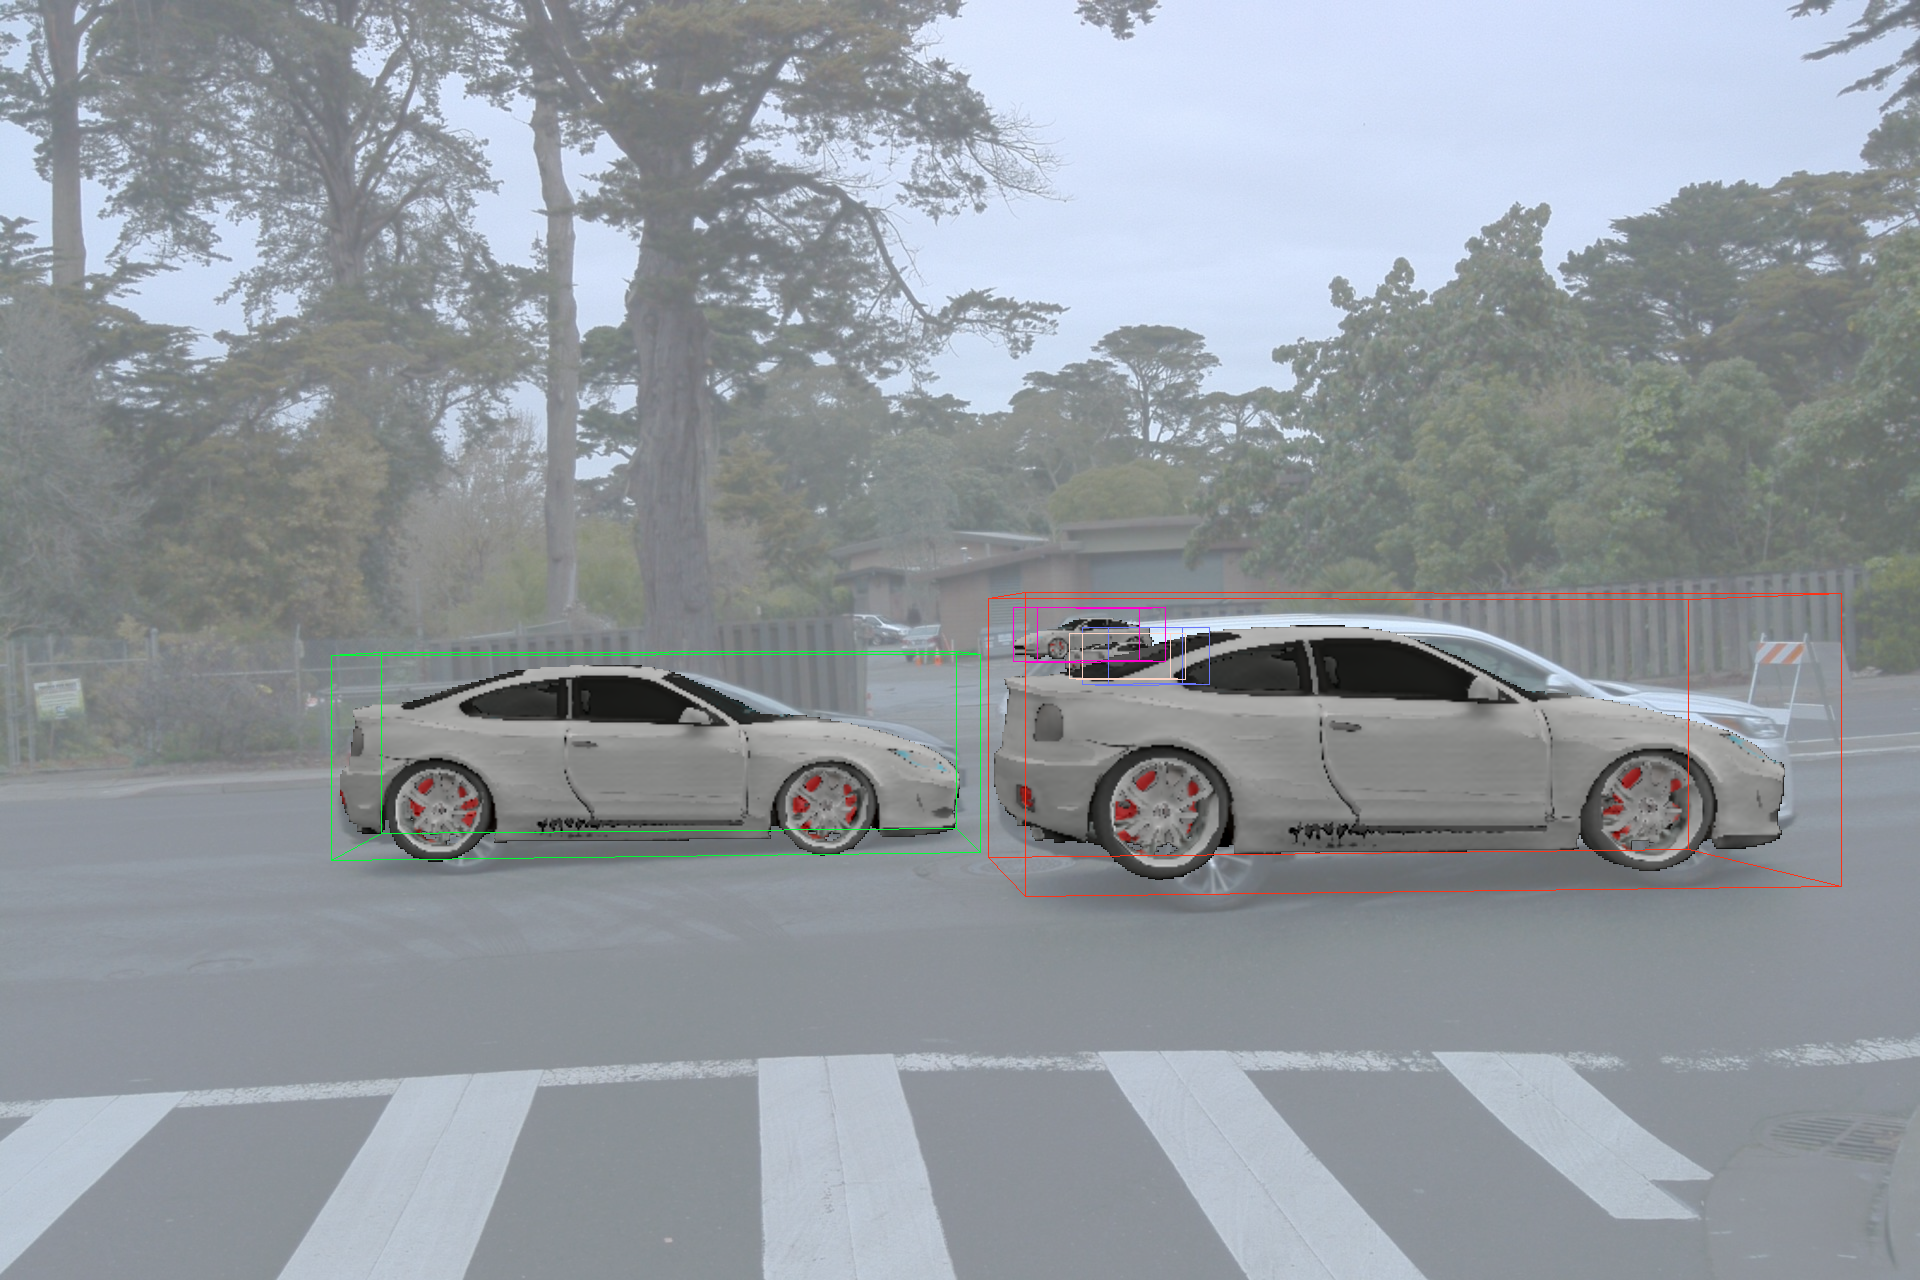
\includegraphics[width=.44\columnwidth, trim={0cm 0cm 0cm 0cm},clip]{fig/optim_supplement/scene11_104/init.png}&
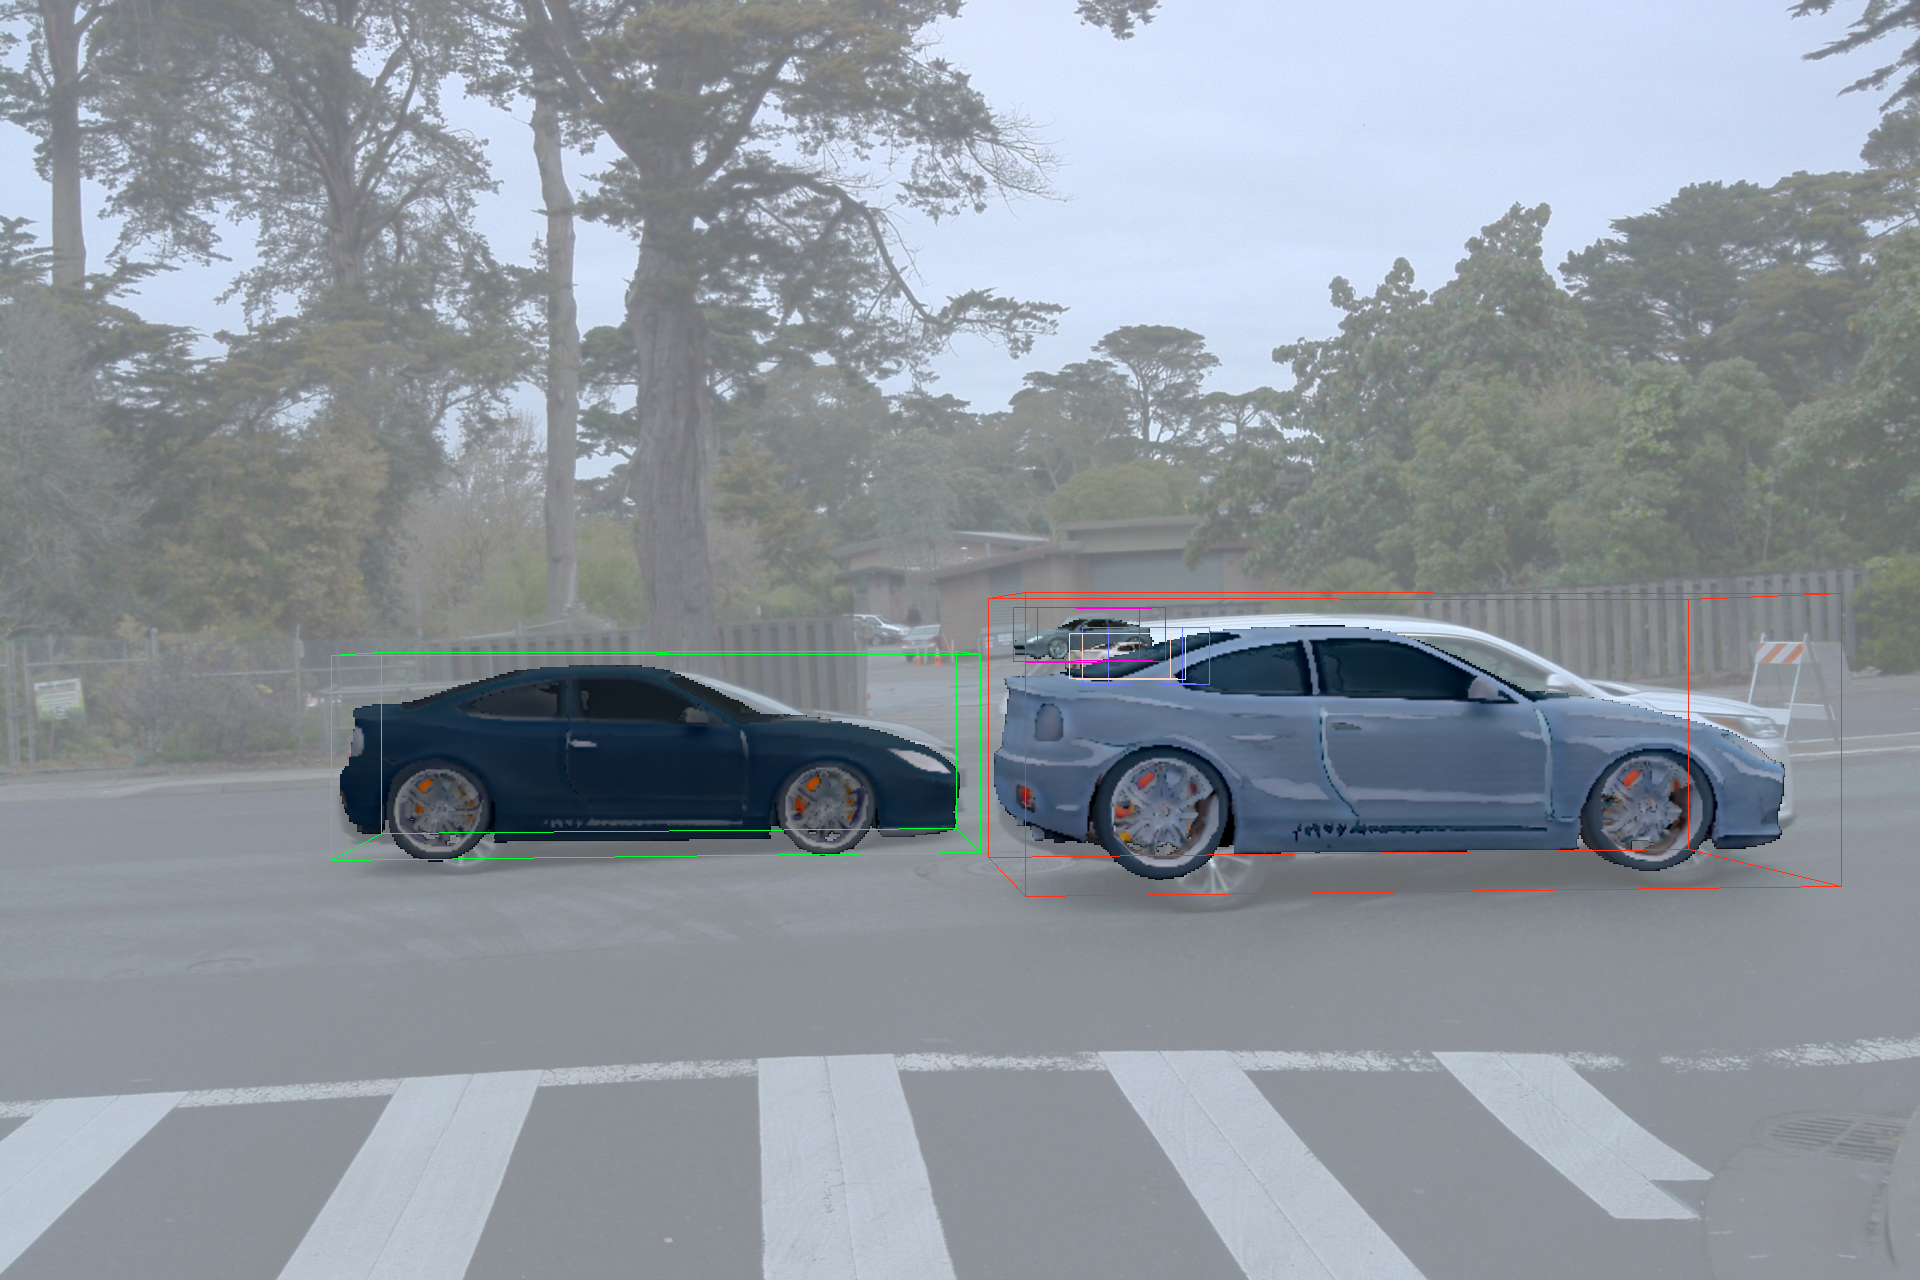
\includegraphics[width=.44\columnwidth, trim={0cm 0cm 0cm 0cm},clip]{fig/optim_supplement/scene11_104/3.png}&
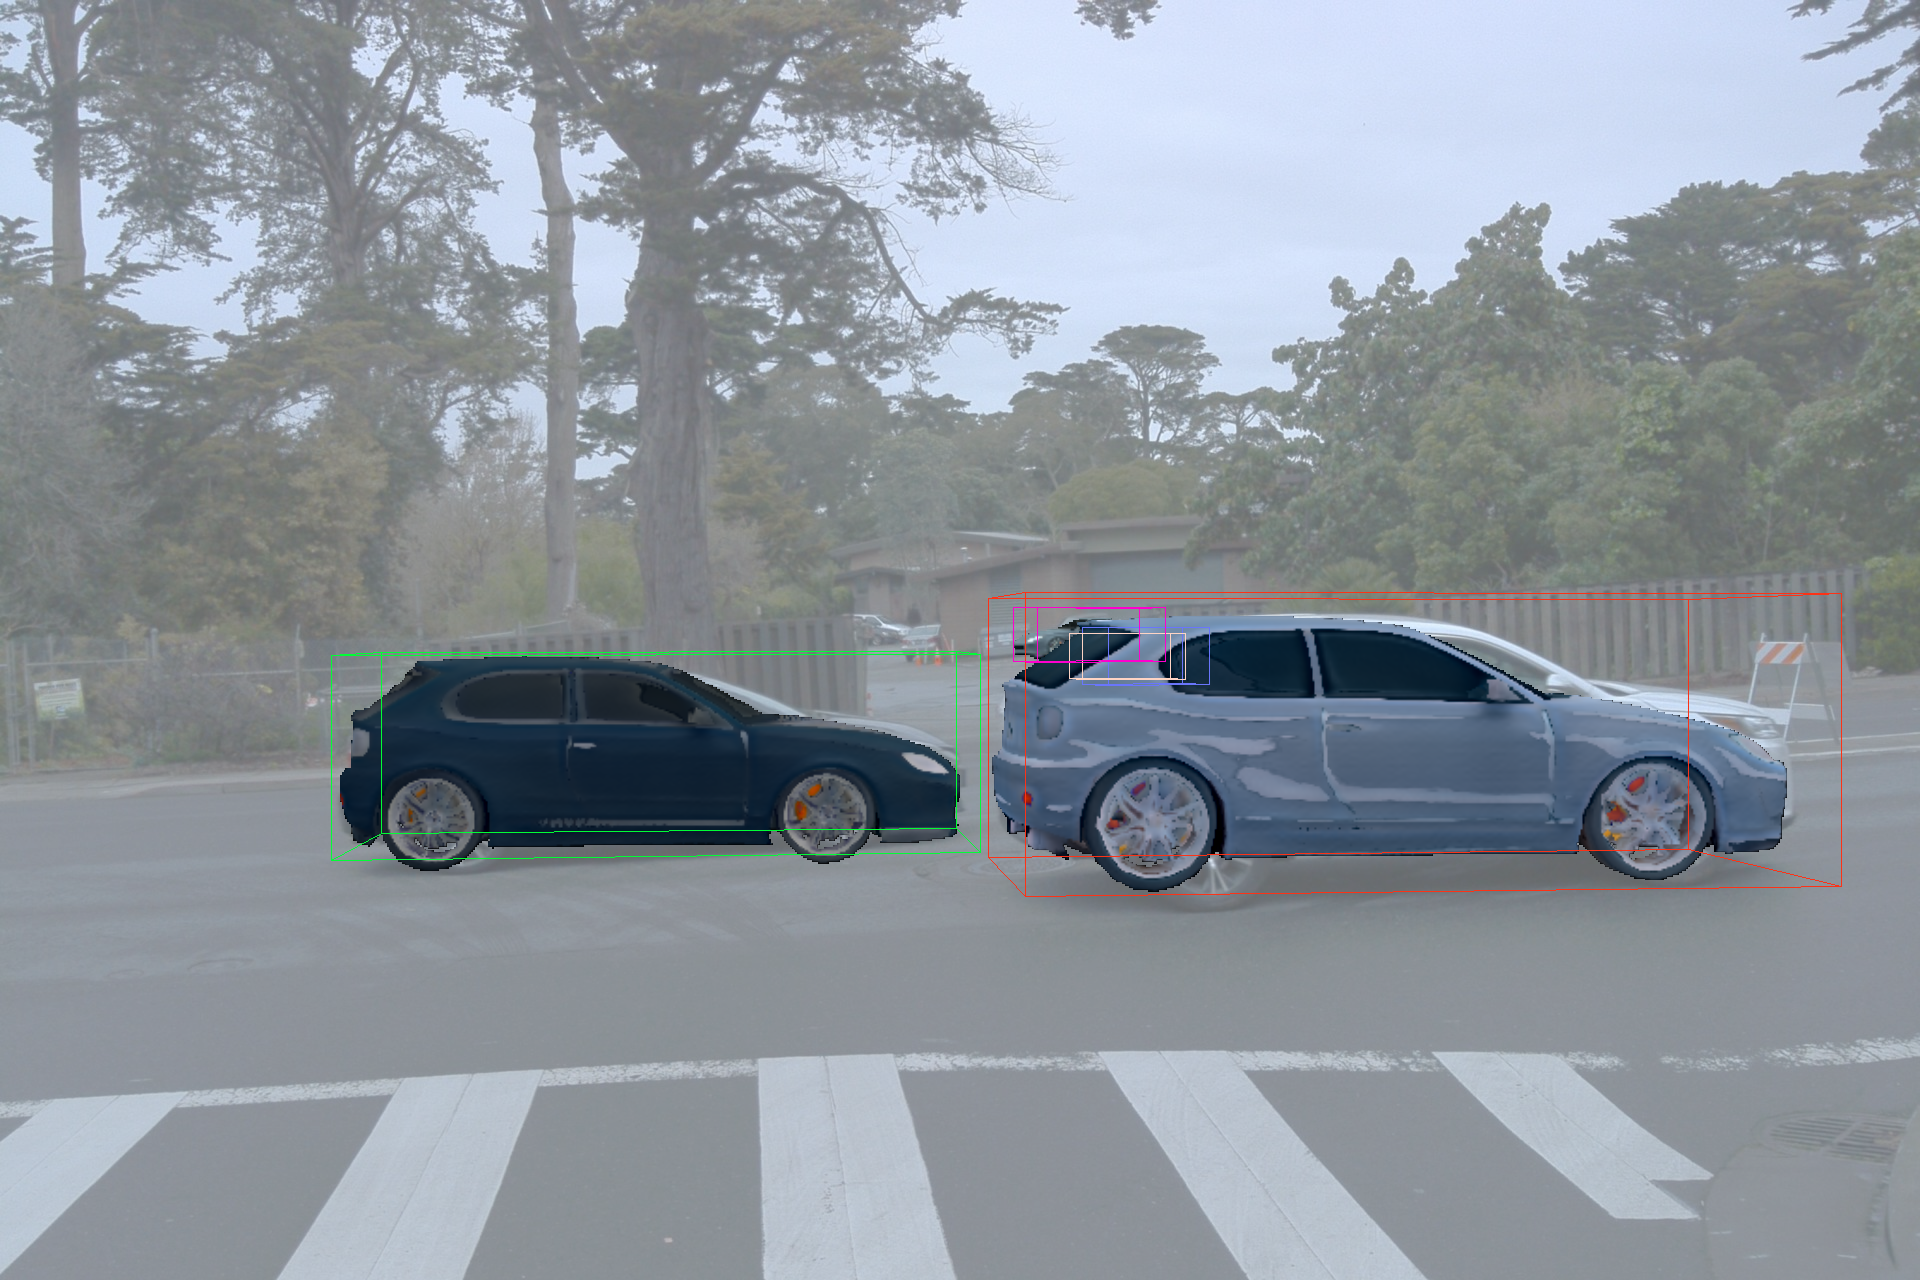
\includegraphics[width=.44\columnwidth, trim={0cm 0cm 0cm 0cm},clip]{fig/optim_supplement/scene11_104/4.png}&
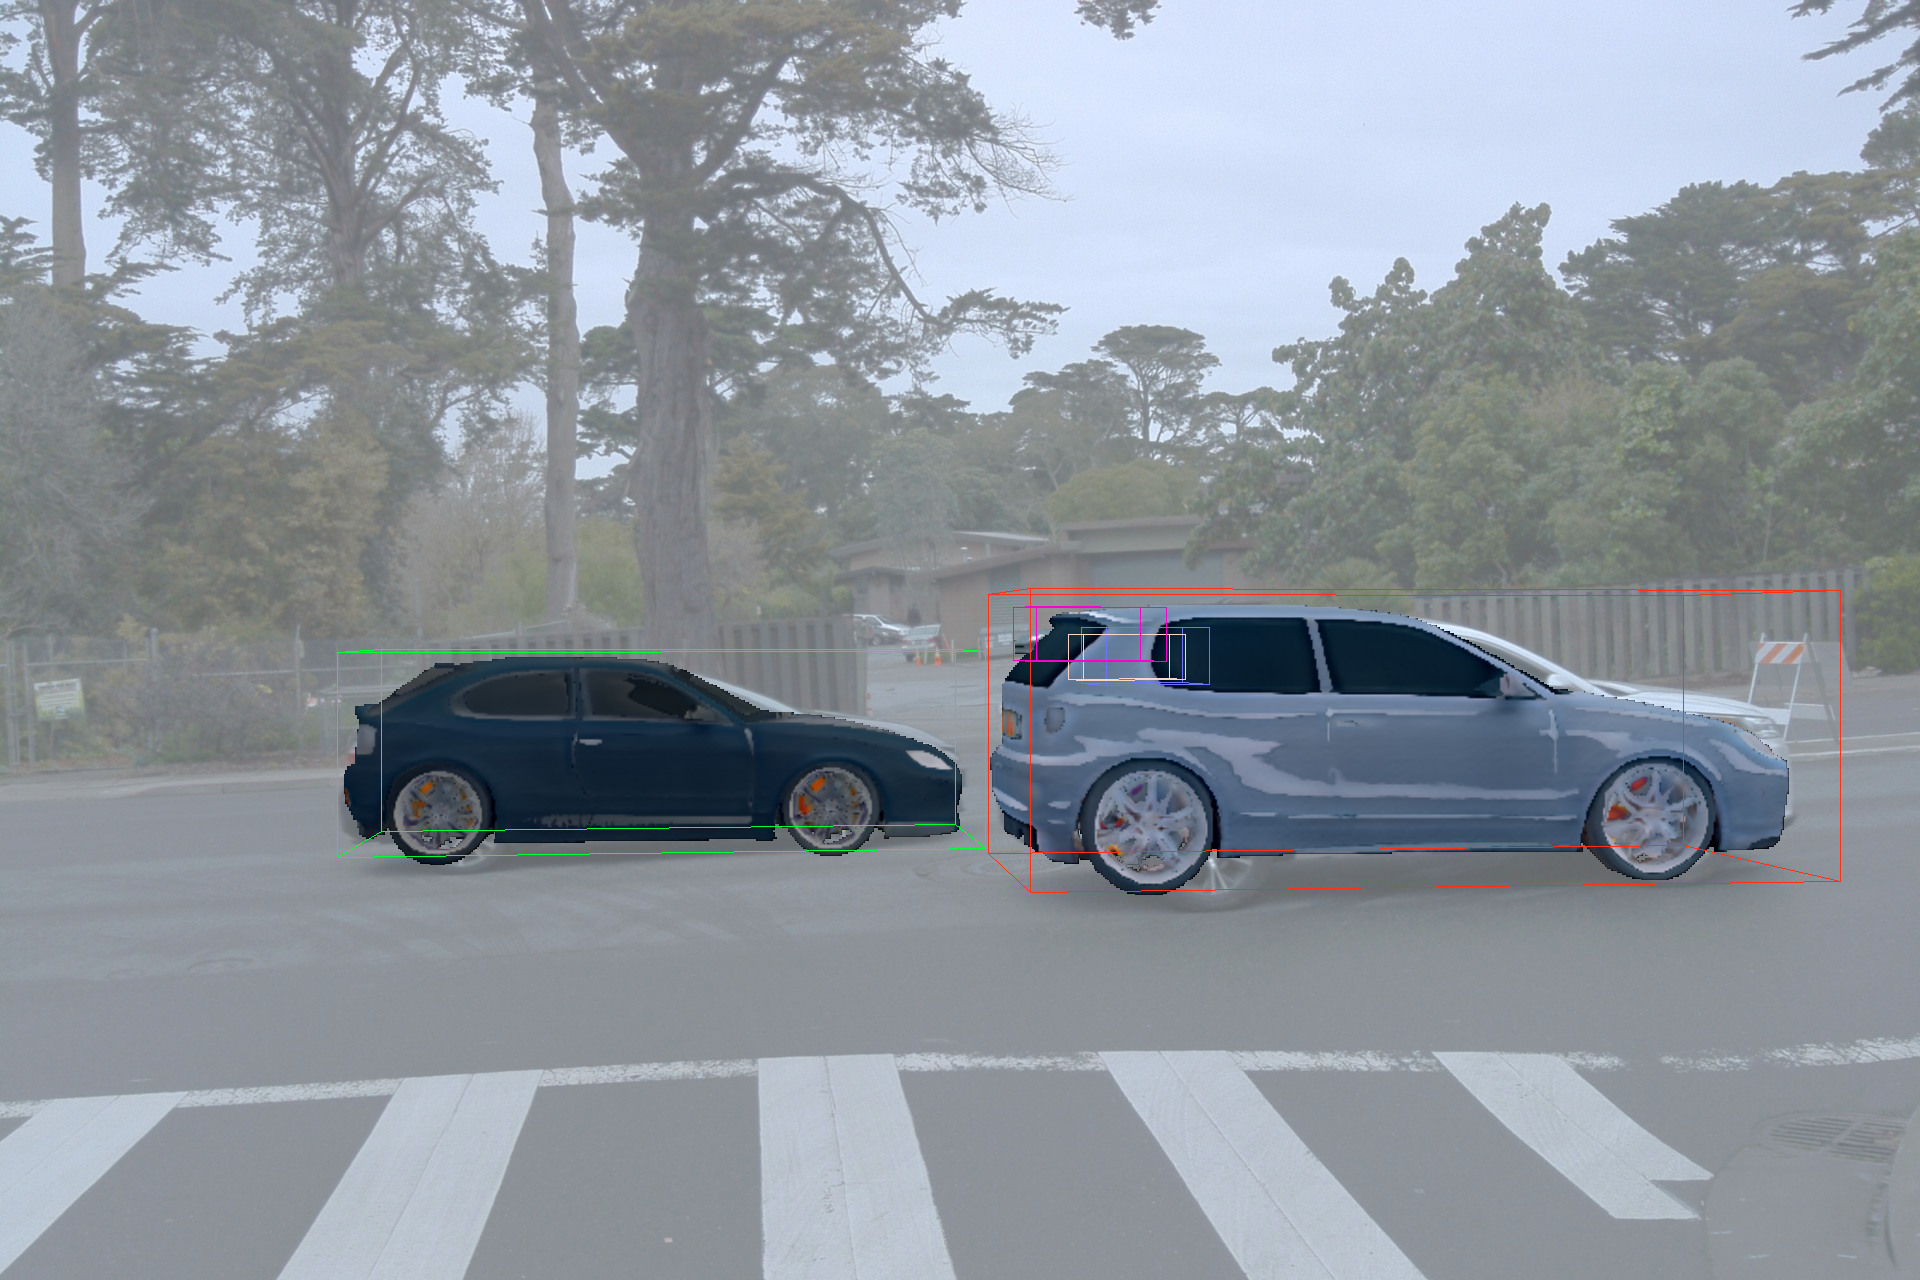
\includegraphics[width=.44\columnwidth, trim={0cm 0cm 0cm 0cm},clip]{fig/optim_supplement/scene11_104/5.png}





\end{tabular}}\vspace*{-6pt}
\caption{\textbf{Optimization Process.} From left to right, we show (i) the observed image, (ii) the rendering predicted by the initial starting point latent embeddings, 
(iii) the predicted rendered objects after the texture code is optimized (iv) the predicted rendered objects after the translation, scale, and rotation are optimized, and (v) the predicted rendered objects after the shape latent code is optimized. The ground truth images are faded to show our rendered objects clearly. Our method is capable of refining the predicted texture, pose, and shape over several optimization steps, even if initialized with poses or appearances far from the target -- all corrected through inverse rendering.}
\label{fig:optim}
\vspace{-8pt}
\end{figure*}
\begin{table}[t!]
\centering
\caption{\textbf{Optimization Schedule.} Test time optimization of all object parameters, the shape and texture embeddings $\textbf{z}_S, \textbf{z}_T$, their location $\mathbf{t}$, rotation $\Phi$ in $\mathfrak{so}(3)$ and scale $s$ follows this schedule. First, the texture is fitted in for two steps, followed by a pose adjustment in one step and inverse rendering of the shape, defined by the respective embedding code. Green denotes the optimization of the parameter in the respective step. The learning rates for all optimized parameters are noted in each field.}
\resizebox{0.6\linewidth}{!}{
    \begin{tabular}{|c|c|c|c|c|c|}
        \hline
         \diagbox[width=\dimexpr \textwidth/3+7\tabcolsep\relax, height=1cm]{\small Step}{\footnotesize Parameter (learning \\ rate)} & $\mathbf{z}_S$ & $\mathbf{z}_T$  & $\mathbf{t}$ & $\Phi$ & $s$ \\
         \hline \hline
         1 & - & \cellcolor{green!25} \num{3e-1} & - & - & - \\ \hline
         2 & - & \cellcolor{green!25} \num{3e-1} & - & - & - \\ \hline
         3 & \cellcolor{green!25} \num{6e-2} & \cellcolor{green!25} \num{3e-1} & \cellcolor{green!25} \num{3e-2} & \cellcolor{green!25} \num{3e-2} & \cellcolor{green!25} \num{1e-6} \\ \hline
         4 & \cellcolor{green!25} \num{6e-2} & - & - & - & -\\ \hline
         5 &\cellcolor{green!25} \num{6e-2} & - & - & - & -\\ \hline
         6 &\cellcolor{green!25} \num{6e-2} & - & - & - & -\\ \hline
    \end{tabular}
}
\label{tab:schedule}
\end{table}


\subsection{Tracking Heuristics}
%
The main paper describes the integration of test-time optimized object representations through inverse rendering into the tracking pipeline. Specifically, Eq.~(6) in the main paper defines the following affinity
\begin{equation}\label{eq:affinity}
    A = w_{IoU} A_{IoU} + w_{z} A_{z} + w_{c} D_{centroid},
\end{equation}
that describes the similarity of tracked and detected objects in the matching step. We follow~\cite{caesar2020nuscenes, weng2020AB3DMOT} and assign $0$ to all object pairs whose center is more than $10m$ apart. In all other cases, we apply the weights $w_{IoU} = 0.7$, $w_{z} = 0.4$, and $w_{c} = 0.5$ between different affinity parameters. Here, $A_{IoU}$ is the true 3D IoU of the bounding boxes, which is computed with the efficient PyTorch3D~\cite{ravi2020pytorch3d} implementation. The affinity $A_{z}$ is computed as the pair-wise cosine distance between all tracklet-detection pairs. 
Centroid distances between pairs are computed in addition to the IoU to compensate for larger errors in line with the camera axis, common in vision-based object detectors. In such cases, IoU might be low, but object distances are still in a reasonable range which we empirically found at $5m$ for the object detector used. Finally, we define the distance-based affinity score as 
\begin{equation}
    D_{centroid} = \text{maximum}\left( \frac{-\| \mathbf{t}_{tracklet} - {t}_{detection} \|_2}{d_{max}}, 0\right) \text{ , with $d_{max} = 5 m$}.
\end{equation}
%
Matches below the threshold of $0.48$ for their affinity score are not considered matched and the respective tracklet is set to ``lost'' and the detection is added as a new tracklet in the next step. Tracklets are considered ``dead'' and removed after a maximum of 4 consecutive lost steps.


\subsection{Details on Generative Object Model}
%
The object generator, used as the prior for car representation, follows the architecture from GET3D~\cite{gao2022get3d}. The generator maps two sample codes $z_{tex}$ and $z_{geo}$, drawn from a Gaussian distribution for the texture and shape respectively, to samples of a 3D SDF and a texture field. Details of this object model's architecture, training, and usage are given below.

\subsubsection{Generator Architecture.} In this work, we employ a variant described in the appendix of~\cite{gao2022get3d}. Following~\cite{karras2019styleGAN,karras2020styleGAN2}, two Gaussian variables are mapped independently to intermediate style embedding $\boldmath{w}_S$ and $\boldmath{w}_T$ in a learned $\boldmath{W}\text{-space}$. Style embeddings are then used as an input to the CNN-based StyleGAN2~\cite{karras2020styleGAN2} generator. Both style embeddings for shape and texture jointly condition the generator in each block, allowing texture and shape to influence the other modality. Each intermediate feature map of the generator backbone is mapped to its respective modality through a mapping layer only conditioned on the respective style embedding. All feature maps are accumulated and reshaped into three feature planes in the last generator layer. These planes represent textures as texture fields, object shapes as Signed Distance Fields (SDFs), and vertex offsets of a corresponding mesh. This forms a feature volume representation of the textured 3D object on two tri-planes. 


% Specifically, the architecture is split into two components: (i) a geometry branch that differentiable outputs a surface mesh of arbitrary topology, and (ii) a texture branch that generates a texture field that can be queried at the surface points to produce colors.

% \subsubsection{Latent space mapping}
% \subsubsection{Tri-plane generator}

\subsubsection{Rendering.} We employ the differentiable marching tetrahedra~\cite{shen2021dmtet} method and extract a mesh representation from the SDF and vertex offsets, allowing more efficient rendering compared to sampling-based volumetric SDF rendering. Differentiable rasterization for meshes efficiently renders a 2D image of the respective mesh. By querying the texture field only at visible surface points, the respective vertex color can be efficiently retrieved to render the RGB image output.

\subsubsection{Training.} The model is trained using adversarial losses defined on the 2D renderings of 3D objects from the ShapeNet version 1 dataset~\cite{shapenet2015}. Specifically, we use a differentiable rasterizer to render RGB images together with the silhouette masks of the objects as in~\cite{gao2022get3d}  with a training configuration that largely follows StyleGAN2 \cite{karras2020styleGAN2} including using a minibatch standard deviation in the discriminator, exponential moving average for the generator, non-saturating logistic loss, and R1 regularization. %The training hyperparameters are also borrowed from StyleGAN2 \cite{karras2020styleGAN2}. 